% ******************************* PhD Thesis Template **************************
\documentclass[a4paper,12pt,times,numbered,print,index,oneside]{Classes/PhDThesisPSnPDF}
% UTRC footer 
%\cfoot{this document contains technical data subject to EU NLR}%
% ******************************************************************************
% ******************************* Class Options ********************************
% ******************************************************************************
% `a4paper' or `a5paper': A4 or A5 Paper size
%
% `11pt' or `12pt'(default): Font Size 10pt is NOT recommended by the University
% guidelines
%
% `oneside' or `twoside'(default): Printing double side (twoside) or single
% side.
%
% `print': Use `print' for print version with appropriate margins and page
% layout. Leaving the options field blank will activate Online version.
%
% `index': For index at the end of the thesis
%
% `draftclassic': For draft mode without loading any images (same as draft in book)
%
% `draft': Special draft mode with line numbers, images, and water mark with
% timestamp and custom text. Position of the text can also be modified.
%
% `abstract': To generate only the title page and abstract page with
% dissertation title and name, to submit to the Student Registry
%
% `chapter`: This option enables only the specified chapter and it's references
%  Useful for review and corrections.
%
% ************************* Custom Page Margins ********************************
%
% `custommargin`: Use `custommargin' in options to activate custom page margins,
% which can be defined in the preamble.tex. Custom margin will override
% print/online margin setup.
%
% *********************** Choosing the Fonts in Class Options ******************
%
% `times' : Times font with math support. (The Cambridge University guidelines
% recommend using times)
%
% `fourier': Utopia Font with Fourier Math font (Font has to be installed)
%            It's a free font.
%
% `customfont': Use `customfont' option in the document class and load the
% package in the preamble.tex
%
% default or leave empty: `Latin Modern' font will be loaded.
%
% ********************** Choosing the Bibliography style ***********************
%
% `authoryear': For author-year citation eg., Krishna (2013)
%
% `numbered': (Default Option) For numbered and sorted citation e.g., [1,5,2]
%
% `custombib': Define your own bibliography style in the `preamble.tex' file.
%              `\RequirePackage[square, sort, numbers, authoryear]{natbib}'.
%              This can be also used to load biblatex instead of natbib
%              (See Preamble)
%
% **************************** Choosing the Page Style *************************
%
% `default (leave empty)': For Page Numbers in Header (Left Even, Right Odd) and
% Chapter Name in Header (Right Even) and Section Name (Left Odd). Blank Footer.
%
% `PageStyleI': Chapter Name next & Page Number on Even Side (Left Even).
% Section Name & Page Number in Header on Odd Side (Right Odd). Footer is empty.
%
% `PageStyleII': Chapter Name on Even Side (Left Even) in Header. Section Number
% and Section Name in Header on Odd Side (Right Odd). Page numbering in footer
%
% ********************************** Preamble **********************************

% Preamble: Contains packages and user-defined commands and settings
% ******************************************************************************
% ****************************** Custom Margin *********************************

% Add `custommargin' in the document class options to use this section
% Set {innerside margin / outerside margin / topmargin / bottom margin}  and
% other page dimensions
\ifsetCustomMargin
  \RequirePackage[left=37mm,right=30mm,top=35mm,bottom=30mm]{geometry}
  \setFancyHdr % To apply fancy header after geometry package is loaded
\fi

% Add spaces between paragraphs
%\setlength{\parskip}{0.5em}
% Ragged bottom avoids extra whitespaces between paragraphs
\raggedbottom
% To remove the excess top spacing for enumeration, list and description
%\usepackage{enumitem}
%\setlist[enumerate,itemize,description]{topsep=0em}

% *****************************************************************************
% ******************* Fonts (like different typewriter fonts etc.)*************

% Add `customfont' in the document class option to use this section

\ifsetCustomFont
  % Set your custom font here and use `customfont' in options. Leave empty to
  % load computer modern font (default LaTeX font).
  %\RequirePackage{helvet}

  % For use with XeLaTeX
  %  \setmainfont[
  %    Path              = ./libertine/opentype/,
  %    Extension         = .otf,
  %    UprightFont = LinLibertine_R,
  %    BoldFont = LinLibertine_RZ, % Linux Libertine O Regular Semibold
  %    ItalicFont = LinLibertine_RI,
  %    BoldItalicFont = LinLibertine_RZI, % Linux Libertine O Regular Semibold Italic
  %  ]
  %  {libertine}
  %  % load font from system font
  %  \newfontfamily\libertinesystemfont{Linux Libertine O}
\fi

% *****************************************************************************
% **************************** Custom Packages ********************************
\usepackage{mathtools}
\usepackage{amsthm}
\usepackage{wasysym}
\usepackage{euscript}

% ************************* Algorithms and Pseudocode **************************

\usepackage{algpseudocode}
\usepackage[final]{listings}

\definecolor{codegreen}{rgb}{0,0.6,0}
\definecolor{codegray}{rgb}{0.5,0.5,0.5}
\definecolor{codepurple}{rgb}{0.58,0,0.82}
\definecolor{backcolour}{rgb}{0.95,0.95,0.92}
 
\lstdefinestyle{customstyle}{
    backgroundcolor=\color{backcolour},   
    commentstyle=\color{codegreen},
    keywordstyle=\color{magenta},
    numberstyle=\tiny\color{codegray},
    stringstyle=\color{codepurple},
    basicstyle=\footnotesize,
    breakatwhitespace=false,         
    breaklines=true,                 
    captionpos=b,                    
    keepspaces=true,                 
    numbers=left,                    
    numbersep=5pt,                  
    showspaces=false,                
    showstringspaces=false,
    showtabs=false,                  
    tabsize=2
}
 
\lstset{style=customstyle}


% ********************Captions and Hyperreferencing / URL **********************

% Captions: This makes captions of figures use a boldfaced small font.
%\RequirePackage[small,bf]{caption}

\RequirePackage[labelsep=space,tableposition=top]{caption}
\renewcommand{\figurename}{Fig.} %to support older versions of captions.sty


% *************************** Graphics and figures *****************************

%\usepackage{rotating}
%\usepackage{wrapfig}

% Uncomment the following two lines to force Latex to place the figure.
% Use [H] when including graphics. Note 'H' instead of 'h'
%\usepackage{float}
%\restylefloat{figure}

% Subcaption package is also available in the sty folder you can use that by
% uncommenting the following line
% This is for people stuck with older versions of texlive
%\usepackage{sty/caption/subcaption}
\usepackage{subcaption}

% ********************************** Tables ************************************
\usepackage{booktabs} % For professional looking tables
\usepackage{multirow}

%\usepackage{multicol}
%\usepackage{longtable}
%\usepackage{tabularx}


% *********************************** SI Units *********************************
\usepackage{siunitx} % use this package module for SI units


% ******************************* Line Spacing *********************************

% Choose linespacing as appropriate. Default is one-half line spacing as per the
% University guidelines

% \doublespacing
% \onehalfspacing
% \singlespacing


% ************************ Formatting / Footnote *******************************

% Don't break enumeration (etc.) across pages in an ugly manner (default 10000)
%\clubpenalty=500
%\widowpenalty=500

%\usepackage[perpage]{footmisc} %Range of footnote options

\usepackage[usestackEOL]{stackengine}

% *****************************************************************************
% *************************** Bibliography  and References ********************

%\usepackage{cleveref} %Referencing without need to explicitly state fig /table

% Add `custombib' in the document class option to use this section
\ifuseCustomBib
   \RequirePackage[square, sort, numbers, authoryear]{natbib} % CustomBib

% If you would like to use biblatex for your reference management, as opposed to the default `natbibpackage` pass the option `custombib` in the document class. Comment out the previous line to make sure you don't load the natbib package. Uncomment the following lines and specify the location of references.bib file

%\RequirePackage[backend=biber, style=numeric-comp, citestyle=numeric, sorting=nty, natbib=true]{biblatex}
%\bibliography{References/references} %Location of references.bib only for biblatex

\fi

% changes the default name `Bibliography` -> `References'
\renewcommand{\bibname}{References}


% ******************************************************************************
% ************************* User Defined Commands ******************************
% ******************************************************************************

% *********** To change the name of Table of Contents / LOF and LOT ************

\newcommand{\TP}[1]{$\text{TP}_{#1}$} % PikeOS Time Partitions
\newcommand{\pctext}[2]{\text{\parbox{#1}{\centering #2}}}
\newtheorem{theorem}{Theorem}[section]
\newtheorem{corollary}{Corollary}[theorem]
\newtheorem{lemma}[theorem]{Lemma}
%\renewcommand{\contentsname}{My Table of Contents}
%\renewcommand{\listfigurename}{My List of Figures}
%\renewcommand{\listtablename}{My List of Tables}


% ********************** TOC depth and numbering depth *************************

\setcounter{secnumdepth}{3}
\setcounter{tocdepth}{2}


% ******************************* Nomenclature *********************************

% To change the name of the Nomenclature section, uncomment the following line
\renewcommand{\nomname}{Glossary}

% ********************************* Appendix ***********************************

% The default value of both \appendixtocname and \appendixpagename is `Appendices'. These names can all be changed via:

%\renewcommand{\appendixtocname}{List of appendices}
%\renewcommand{\appendixname}{Appndx}

% *********************** Configure Draft Mode **********************************

% Uncomment to disable figures in `draft'
%\setkeys{Gin}{draft=true}  % set draft to false to enable figures in `draft'

% These options are active only during the draft mode
% Default text is "Draft"
%\SetDraftText{DRAFT}

% Default Watermark location is top. Location (top/bottom)
%\SetDraftWMPosition{bottom}

% Draft Version - default is v1.0
\SetDraftVersion{v1.1}

% Draft Text grayscale value (should be between 0-black and 1-white)
% Default value is 0.75
%\SetDraftGrayScale{0.8}


% ******************************** Todo Notes **********************************
%% Uncomment the following lines to have todonotes.

\ifsetDraft
	\usepackage[colorinlistoftodos]{todonotes}
	\newcommand{\todonote}[1]{\todo[size=\small,inline,color=green!40]{#1}}
\else
	\newcommand{\todonote}[1]{}
	\newcommand{\listoftodos}{}
\fi

% Example todo: \mynote{Hey! I have a note}

% **************************** Other custom commands *****************************


% ************************ Thesis Information & Meta-data **********************
% Thesis title and author information, refernce file for biblatex
% ************************ Thesis Information & Meta-data **********************
%% The title of the thesis
\title{From natural language requirements to Simulation Monitors: Synthesis through code generation}
%Automatic Code Generation for Embedded Multi-Core systems for Mixed Criticality Applications 

%\texorpdfstring is used for PDF metadata. Usage:
%\texorpdfstring{LaTeX_Version}{PDF Version (non-latex)} eg.,
%\texorpdfstring{$sigma$}{sigma}

%% Subtitle (Optional)
%\subtitle{Using the LateX template}

%% The full name of the author
\author{Marco Emanuele Celia}

%% University 
\university{University of Pisa, Scuola Superiore Sant'Anna}
%% Department (eg. Department of Engineering, Maths, Physics)
\dept{Information Engineering Department\\ Institute of Communication, Information and Perception Technologies}

% University crest
% Crest minimum should be 30mm.
\crest{
\includegraphics[width=0.3\textwidth]{UniversityCrest}}
%% Use this crest, if you are using the college crest
%% Crest long miminum should be 65mm
%\crest{\includegraphics[width=0.45\textwidth]{University_Crest_Long}}

%% College shield [optional] 
% Crest minimum should be 30mm.
\collegeshield{
\includegraphics[width=0.2\textwidth]{UniversityCrest}}


%% Supervisor (optional)
%% for multiple supervisors, append each supervisor with the \newline command
\supervisor{Prof. Marco Di Natale\\Prof. Giorgio C. Buttazzo}
\extsupervisor{Dr. Stylianos Basagiannis}

%% Supervisor Role (optional) - Supervisor (default) or advisor
% \supervisorrole{\textbf{Supervisors: }}
%% if no title is desired:
% \supervisorrole{}

%% Supervisor line width: required to align supervisors
%\supervisorlinewidth{0.35\textwidth}

%% Advisor (optional)
%% for multiple advisors, append each advisor with the \newline command
%\advisor{Dr. A. Advisor\newline
%Dr. B. Advisor}
     
%% Advisor Role (optional) - Advisor (default) or leave empty
% \advisorrole{Advisors: }
%% if no title is required
% \advisorrole{}

%% Advisor line width: required to align supervisors
%\advisorlinewidth{0.25\textwidth}


%% The submission text:
\renewcommand{\submissiontext}{Master Degree in Embedded Computing Systems}
%% Full title of the Degree
%\degreetitle{Embedded Computing Systems}

%% College affiliation (optional)
\college{University of Pisa}
%% Submission date
% Default is set as {\monthname[\the\month]\space\the\year}
\degreedate{July 2017} 

%% Meta information
\subject{Master thesis} \keywords{{Mix-criticality}{Embedded} {Code Generation} {Simulink} {Scuola Superiore Sant'Anna}}


% ***************************** Abstract Separate ******************************
% To printout only the titlepage and the abstract with the PhD title and the
% author name for submission to the Student Registry, use the `abstract' option in
% the document class.

%\ifdefineAbstract
 %\pagestyle{empty}
 %\includeonly{Abstract/abstract}
%\fi

% ***************************** Chapter Mode ***********************************
% The chapter mode allows user to only print particular chapters with references
% Title, Contents, Frontmatter are disabled by default
% Useful option to review a particular chapter or to send it to supervisior.
% To use choose `chapter' option in the document class

%\ifdefineChapter
% \includeonly{Chapter3/chapter3}
%\fi

% ******************************** Front Matter ********************************

\begin{document}


\frontmatter

\maketitle

% ******************************* Thesis Dedidcation ********************************

\begin{dedication} 



\end{dedication}


% ************************** Thesis Acknowledgements **************************

\begin{acknowledgements}      

Without the effort of several people this work wouldn't be possible. First of all, I would like to thank my supervisor, Marco Di Natale, for having introduced me into the world of the Model-Based Design, for being always available to answer my questions and clarify my doubts and, most important, for his precious life teachings.

\paragraph{} I would like to thank United Technologies Research Center for the big opportunity they gave to me. In this six months I experienced a professional and high qualified environment. I have been really surprised on how employees are considered to be the most important resource to achieve their purposes. A special thank to Vassilios Tsachouridis who really made me capable to deal with the complexity of Control Systems. I consider myself very lucky for having worked with him. Thank also to Stylianos Basagiannis who always watched over me and ensured of my wellness. Lastly, thank to the rest of the team, Juan Valverde and Georgeos Giantamidis for the hard work and the funny moments.

\paragraph{} I would like to mention also people who indirectly contributed to this work.
\\
\textit{Un ringraziamento speciale ai miei amici per non avermi mai fatto mancare il loro aiuto, con le parole e, soprattutto, con i fatti. Senza il contributo di ciascuno di voi non sarei arrivato a questo traguardo.
\\
Grazie a Miriam per essermi stata accanto in questi anni, per avermi sopportato e avermi sempre offerto una via di fuga dai miei pensieri.
\\
Infine, grazie alla mia famiglia per non avermi mai fatto mancare il loro supporto e la loro fiducia.}

{\raggedleft\vfill\itshape\Longstack[l]{
  Marco Celia\\
  Cork, July 2017
}\par
}


\end{acknowledgements}

% ************************** Thesis Abstract *****************************
\begin{abstract}
The increasing level of complexity of modern embedded systems concurs to enhance the gap between the textual representation of High-Level System Requirements and the testing units in charge of their verification. Such gap is worsened by the possible presence of errors and omissions in the natural language requirement and causes engineers to inject into the verification units features derived from their personal interpretation.
 
The goal of this Master thesis is to provide a framework consisting of a requirement (loose) syntax, a requirements editor, a parser, and an automatic synthesis tool, which helps engineers writing high level requirements in a structured natural language with a contract-based paradigm, thus reducing, as much as possible, inconsistency and common errors, and directly generating verification monitors for a target platform.
 
To restrict the domain and the framework complexity and make the problem affordable, the first version of the tool is restricted to the controls domain and assumes the use of Simulink as a modelling and simulation tool. To ease the generation process, a control verification Simulink library has been implemented.
\end{abstract}


% *********************** Adding TOC and List of Figures ***********************

\tableofcontents
\listoffigures
%\listoftables

% \printnomenclature[space] space can be set as 2em between symbol and description
\setlength{\nomitemsep}{0.1em}
\printnomenclature[1cm]

% ******************************** Main Matter *********************************
\mainmatter
%!TEX root = ../thesis.tex

\chapter{Introduction}


%\ifpdf
 %   \graphicspath{{Chapters/Figs/Raster/}{Chapters/Figs/PDF/}{Chapters/Figs/}}
%\else
%    \graphicspath{{Chapters/Figs/Vector/}{Chapters/Figs/}}
%\fi


%********************************** % Section  **************************************
\section{Development Models}
\label{sec:devmodels}


Every industrial product has its own \textit{life-cycle} which starts when comes out the need of a new product and continues with the requirements identification, design, development and verification processes. Furthermore several other activities regarding the product maintenance could be as well part of the cycle. There are several approaches describing the sequentiality of product life cycle tasks, such as the so called \textit{Waterfall model} (Fig.\ref{fig:waterfall}), in which a phase starts after the completion of the previous one and phases' deliverables follows an unidirectional flows like in a pipeline.
\begin{figure}[!h]
	\centering 
     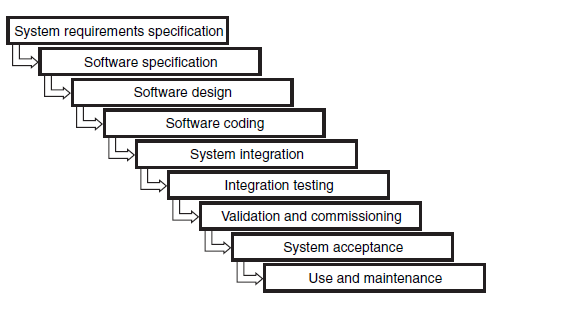
\includegraphics[width=.75\textwidth]{Figs/waterfall.png} 
     \caption{Waterfall Model} 
     \label{fig:waterfall} 
\end{figure} 

A example of the waterfall model we can examine the military standard MIL-STD-2167A, which establish a uniform development model applicable during the whole system life-cycle.
\par As second alternative  the \textit{V-model} (Fig.\ref{fig:vmodel}) enforces the temporal correlation among developing and validation phases. Activities on the left hand side of the V are associated with models of the system, where each subsequent activity represents an enhancement of the model from the previous activity. Processes on the right hand side of the V correspond to experimental (testing) activities. Results of a test phase validate the structure of the correspondent developing phase.

\begin{figure}[!h]
	\centering 
     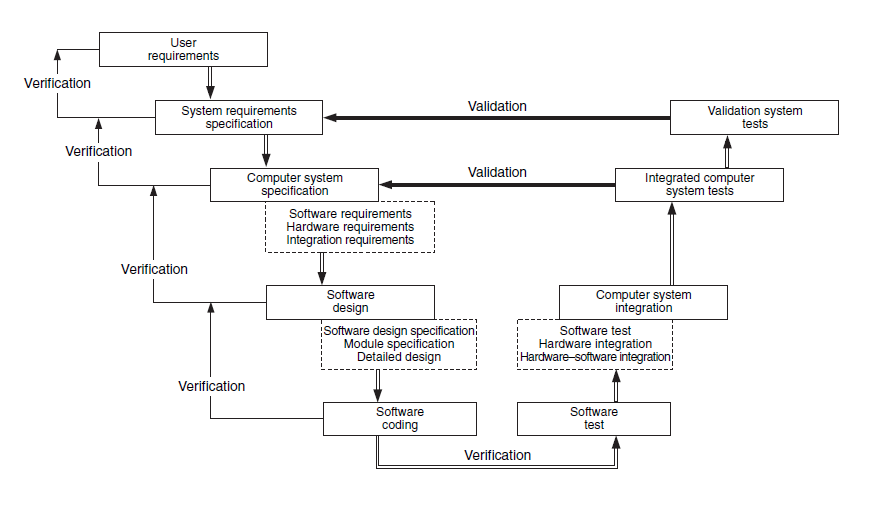
\includegraphics[width=\textwidth]{Figs/vmodel.png} 
     \caption{V-Model} 
     \label{fig:vmodel} 
\end{figure} 

This work focuses on the first stage of a generic product development model, i.e. Requirement analysis, trying to reduce the gap also with its relative validation.

%********************************** % Section  **************************************
\section{Requirements Fundamentals}
\subsection{Definition}
\begin{quote}
"...Requirements definition is a careful assessment of the needs that a system is to fulfill. It must say why a
system is needed, based on current and foreseen conditions, which may be internal operations or an external market. It must say what system features will serve and satisfy this context. And it must say h ow the
system is to be constructed..." — Doug Ross [Ross77a]
\end{quote}
Regardless of the adopted development model, the first, and critical, step to approach a product development is the System Requirement specification. It is much more than a functional specification, it is the groundwork for all the future stages and hence it has to catch everything is needed in terms of performance, behaviors and constraints to be satisfied. 
\par Being the requirement analysis the fundamental step that drives the design and implementation phases it is also worth noting how errors at this stage, \textit{late} errors, are much more costly in terms of time to be fixed than \textit{early} errors. The DoD Software Technology Plan \citep{DoD91} states that "early defect fixes are typically two orders of magnitude cheaper than late defect fixes, and the early requirements and design defects typically leave more serious operational consequences."

\subsection{Guidelines}


The result of the system requirements specification process is an
unambiguous and complete specification document. It should help:
\begin{enumerate}[label=\alph*)]
\item System customers to accurately describe what they wish to obtain;
\item System suppliers to understand exactly what the customer wants;
\end{enumerate}
Furthermore to the stakeholders a good system requirements specification (SRS) should provide several specific benefits, such as the following:
\begin{itemize}[label={--}]
\item \textit{Establish the basis for agreement between the customers and the suppliers on what the software
product is to do}. The complete description of the functions to be performed by the software specified
in the SRS will assist the potential users to determine if the software specified meets their needs or
how the software must be modified to meet their needs
\item \textit{Reduce the development effort}. The preparation of the SRS forces the various concerned groups in
the customer’s organization to consider rigorously all of the requirements before design begins and
reduces later redesign, recoding, and retesting. Careful review of the requirements in the SRS can
reveal omissions, misunderstandings, and inconsistencies early in the development cycle when these
problems are easier to correct.
\item \textit{Provide a baseline for validation and verification.} Organizations can develop their validation and
verification plans much more productively from a good SRS. As a part of the development contract,
the SRS provides a baseline against which compliance can be measured.
\end{itemize}
\par Attempts to reduce as much as possible the inconsistencies coming from the plain text descriptions has been proposed in several standards. The IEEE 830-1998 \citep{ieee1998ieee} offers a metric to produce and evaluate a good system requirements specification in terms of 
\begin{enumerate}[label=\alph*)]
\item Correctness
\item Unambiguity
\item Completeness
\item Consistency
\item Verifiability
\item Modifiability
\item Traceability
\end{enumerate}
while the MIL-STD-498 \citep{united1994mil} was a United States military standard whose purpose was to establish uniform requirements for systems development and documentation. Those standards rather than automatic tools are sort of guidelines to achieve a good specification for the system.

\subsection{Requirement Specification languages}
As said above, the requirement document quite often serves as a "contract" between designers and the costumers, as such it has to be somehow understandable also from those people having a non technical background, so quite often they are given with many pages of natural language descriptions, sometimes flanked with manually derived diagrams that represent the structure of the design. Due to its nature, the natural language specification of a property could be very far, and sometimes totally unrelated, from a formal definition. For instance natural language could be lacking, redundant or misleading, even worse the requirement definition is generally the result of an empirical process subjected to ambiguity, subjectivity and imprecisions.
\par The literature provides several methods aiming to avoid bad-formed requirements, all of them are based on the addition of a certain degree of formality in the syntax used to define the property referring a specific requirement. The most general classification of the specification languages is into \textit{formal}, \textit{semi-formal} and \textit{informal}.
\par A language is formal if its syntax and semantic are defined in a rigorous mathematical way. A formally expressed requirement provides an high level of verifiability, furthermore the process of translating natural into formal language requires the analysts to improve their comprehension of the requirement semantic. In fact, in order for the translation to be successful they have to verify, and eventually eliminate, the presence of ambiguities also from the natural language definition.
\par Semi-formal languages are usually expressed in a graphical manner, aimed to provide a non-ambiguous description through a generally easier syntax that has not a direct mapping to a mathematical semantic. The \textit{structured natural language}, which will be of interest in below discussions, could be in turn part of this category. In particular it could be view as a plain text which has some constraint in the precedence of sentences participants.%ref to UML-SysML??
\par Informal languages are those that have neither a rigorous syntax or rigorous semantic. In particular the syntax is derived from the relative grammatic and the semantic is that rich that makes impossible its formalization. Despite all this, they are the most commonly used, and, hence, a good specification always relies on the experience of designers.

\subsection{Readability versus Formality}
The more we increase the syntax formality and the more the number of possible inconsistencies is reduced. As drawback requirement specification starts taking a non-easy readable shape and becomes very distant from its natural language expression. There are several reasons why this aspect represents an obstacle to the usability of these techniques. First, a requirements document could not be anymore used as sort of contract among stakeholders since there are no guarantees that one of the parts is able to understand the meaning of the formula. Further, their use implies engineer to have a certain level of expertise in typing formal requirements. Although the usability does not constitute the strength of this approach the reason why formal languages are still of interest is due to their capability of totally avoid formulas ambiguity.

\subsection{Requirements Specialization}
A direct consequence of the use of formal languages is the possibility to perform automatic verification techniques out of the requirements, but, as previously said, rarely the specifications are formally written, implying, hence, several manual translation stages from natural language. 
\par This work bridges the gap between formal and informal representation of requirements. In order to do so the effort has been spread along an ideal line starting from the natural up to the formal language description. The first step consists of defining a syntax which allows the presence of free-text, limited to certain points of the sentence, and, at the same time, preserves a well defined structure. Once the requirements are structured is then possible to apply some processing technique able to recognize every \textit{common pattern}, i.e. all those properties having a direct correlation, in terms of temporality or property semantic, with a specific formal language pattern. Finally the formal properties are used to generate automatically verification monitors.
\begin{figure}[!h]
	\centering 
     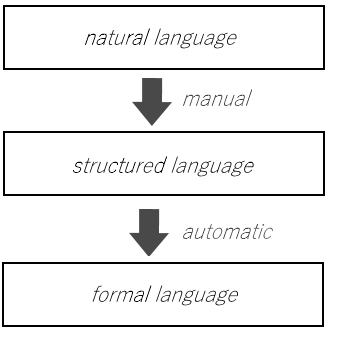
\includegraphics[width=.4\textwidth]{Figs/specialization.png} 
     \caption{Requirement specialization} 
     \label{fig:reqspec} 
\end{figure} 
 
\subsection{High-Level Requirements}
Rarely system requirements are written in a formal language, the non-rigorous nature of plain text constitutes the main obstacle to automatic generation of monitors out of the specification. Writing requirements in a semi-formal shape rather than a plain text will make them suitable to language processing techniques which allow to get their formal specification. As enforcement of this concept, in certain specific application domain requirements usually refer to properties having a well-known semantic. Typically for such cases also plain text requirements tend to have a fixed structure. This scenario commonly recurs when the specification is given from an high level of abstraction of the systems and, hence, does not regard constraints on the development. Performance requirements in a control system are an example. In fact they have an invariant textual form compared, for instance, to system's hardware structure or control algorithms.
%********************************** % Section  **************************************
\section{Verification tools}

\subsection{Property checking}

In general, the problem of determining whether a property $\phi$ is satisfied from system $S$ could be faced in many ways depending on the set of environmental conditions in which system and property are defined. Being not too much formal we can define a system $S$ as an entity that correlates inputs and output signals according to a precise law, while the \textit{model} of the system as a set of possible \textit{states} in which system can lie, each state $x_{i}$ ranging over the domain $X_{i}$. A system evolves over the time domain and the function $\beta :T\rightarrow X$, associating a state to a precise time instant, is called \textit{behavior} of the systems. 
Within this context a property $\phi$ defines a subset of the systems' state and a property \textit{monitor} is that entity that ensures whether a certain behavior \textit{satisfies} the property, i.e. whether $L_{\phi}\in X$.
\par The procedure leading to the verification of a property, or formula, consists of associating a function $\Omega_{\phi}:X\rightarrow B$ which, given the set of all possible behaviors returns a boolean value meaning whether the property is satisfied or not. Behaviors are examined one at time assuming the presence of a simulation unit charged to produce them. 
A monitor is hence another unit which cooperates with the system simulator mainly in three ways (Fig.\ref{fig:monitortypes}). 

\begin{figure}[!h]
	\centering 
     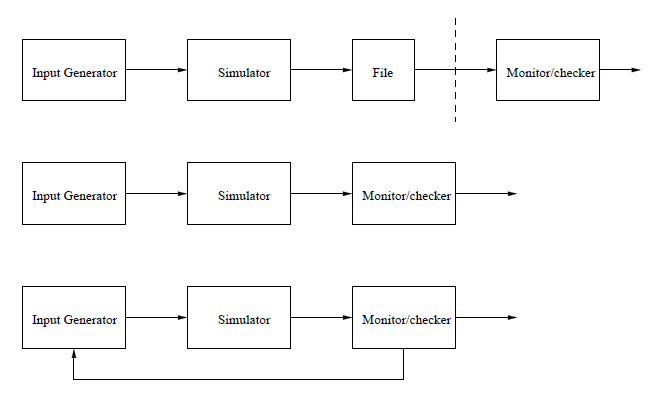
\includegraphics[width=.8\textwidth]{Figs/monitortypes.png} 
     \caption{Off-line, Passive On-line and Active On-line monitors from \citep{maler2008checking}} 
     \label{fig:monitortypes} 
\end{figure} 
The \textit{off-line} monitoring expects monitors to check formulas against the simulation traces. Since monitors are no forced to be causal over the execution time this technique constitutes the easiest way to conduce model checking. In the \textit{on-line} methods the monitor is running in parallel with the simulator, we refer to \textit{active} on-line if the monitor is also affecting, through a feed-back loop, the simulation inputs, and \textit{passive} on-line otherwise. In general on-line monitors have the advantage of being able to assert satisfaction or violation of a property while the simulation is running, this prevents either high time consuming simulation to be terminated and dangerous behavior to occur after the violation of the property. The cost we pay for an on-line monitoring is that formulas must be causal, i.e. it is not possible to check a property at certain time $t$ as function of states occurring later than $t$. Since this work focuses mostly on dynamic controls system domain monitors that are better suited to fit it are of the type passive on-line. 

\subsection{Automatic monitor generation}
Under the assumption that requirements are written in formal language, i.e. absence of inconsistencies, the generation of verification monitors for simulation can be performed in an automatic way. 
\par Code generation procedures are always targeted to a specific platform, which in turn varies as function of the application domain. For what regards dynamical systems typical targets are simulation frameworks such as Simulink by Matworks\citep{Simulink} and LabVIEW\citep{Labview}. Together with the target platform usually code generation starts from a model of the entities we want generate for. 
\par Tools such as Acceleo\citep{acceleo} are based on the prior definition of the mode of the system architecture, allowing language independent code generation from any kind of EMF compatible meta-model, such as UML, UML 2.0 and SysML. Also Simulink with the Embedded Coder offers the possibility to customize the C/C++ code generated from any Simulink model.
\par Another chance is to not rely on the presence of a system model and generate code implementing verification monitors directly from statements expressed in some formal language. The work in \citep{bals2017} starts from properties expressed in the STL formal language\citep{maler2008checking} and produces Simulink monitors, to ease the auto-generation procedure it makes use of a library implementing the STL temporal operators.

\section{Proposed Tool}

\subsection{Premise}
This work aims to show the feasibility of a tool that starts from semi-formal system specification and ends up with verification monitors to be plugged into a simulation model of the system. The number of particular cases to deal with it is huge and the scalability of the approach is a key factor that needs time to be proved. However, due to the impact that such a tool could have in the design and verification processes, the problem has been sized in order to be manageable at least with the purpose of producing a proof of concept prototype.
\par For the above reasons we decide to use, as a case study, the high-level requirements for dynamic control systems. Such requirements has been restructured in the \textit{contract-base} paradigm, which, basically, expect the formulation of the property as a composition of two main sections, \textit{assumption} and \textit{assertion}, were the first logically implies the second.
\par Further the formalization of the requirements has been performed using the STL formal language, which, unlike many others temporal logics derived from LTL, adds some domain specific features that will be better described in sec.\ref{sec:STL}. Finally, as target platform, Simulink has been selected since it is one of the most used simulation tools for such application domain. A graphical representation of the whole framework together with the smart editor, which will be discussed in next section, is presented in figure \ref{fig:framework}.

\begin{figure}[!h]
	\centering 
     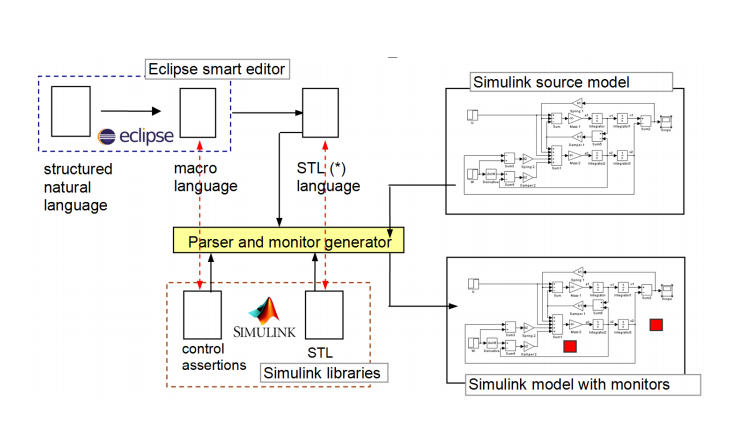
\includegraphics[width=1\textwidth]{Figs/framework.png} 
     \caption{Framework} 
     \label{fig:framework} 
\end{figure}

\subsection{Custom Editor}
The smart editor is meant as the tool helping users to write semi-formal requirements. It has been implemented as an Eclipse Editor plug-in, from which inherits many features common to most commercial editors such as \textit{context-aware} text completion and syntax error checking. The editor comes with it is own syntax which even if for the time being is deeply application domain oriented preserves a modular an easily extensible software structure.
\par Some more specific features are the capability to import a data dictionary which is ideally synchronized with the target model and generate platform dependent monitors. 
\chapter{MDB and Hybrid Systems}

\section{Why models}
\begin{figure}[!h]
	\centering 
     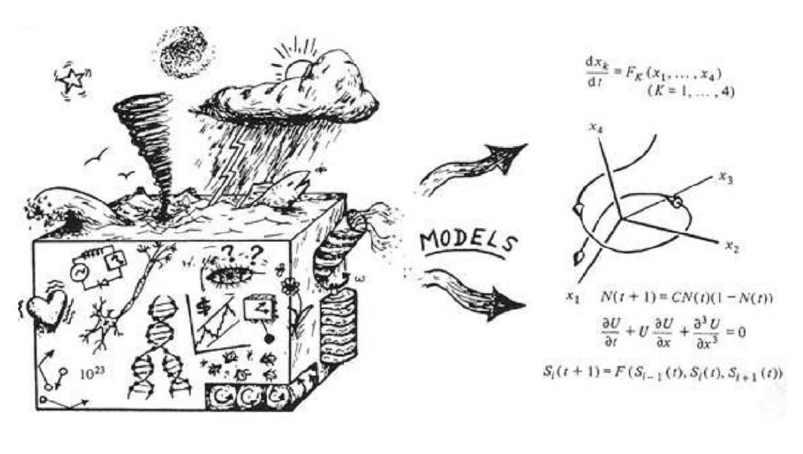
\includegraphics[width=.9\textwidth]{Figs/models.PNG} 
     \caption{Modeling} 
     \label{fig:models} 
\end{figure} 
We can define a model as a simplification of the reality (Fig.\ref{fig:models}). Models can be of any nature, \textit{mathematical models} are, typical, sets of equations, \textit{physical models} could be mock-ups aiming to provide a final picture of what the system will look like and so on.
\par Usually a model is the result of a process affected of different metrics. In a very generic perspective the first is the determination of \textit{model type}, namely which of all the possible approaches, leading to a correct result, to model our system (mathematical, graphical, textual and so on) is the most appropriate one. In practical cases this step translates in choosing the most appropriate modeling tool.
\par The second is the determination of the \textit{level of abstraction} of our model, since any system can be view as a composition of several layers one may be more interested in representing features of some of them. However, a good model has always to be connected enough to reality, indeed the risk to oversimplify may cause the model to lose meaningful information. 
\paragraph{} The previous metrics could be in turn influenced by the \textit{model purpose}. One possible scenario is when industries and organizations wants to shorten as much as possible the development time, the most natural way to accomplish that is to reuse as much as possible what they already have implemented. Reuse always implies knowledge, therefore models can be used to provide graphical and more intuitive documentations for the software or system. This is the case of UML \citep{james1999unified} and SysML\citep{sysml}, the first is a general-purpose visual modeling language that is used to specify, visualize, construct, and document the artifacts of a software system, while the latter was defined as extension of the first and provide support for the specification, analysis, design, verification, and validation of systems that include hardware, software, data, personnel, procedures, and facilities.
\paragraph{} On the other hand there could be many cases in which for a certain application domain, aerospace for instance, fully test the final product before using it's an high costly process. More, sometimes reproducing all the possible testing cases could be either too difficult or too dangerous, just think to nuclear applications. Hence, for all of these reasons, systems models could be used to simulate behavior, perform tests and verify compliance against the design. The methodology considering the model as the primary artifact for simulating the system behavior and verify properties on the behavior is called \textit{Model Based Design}.

\section{Model Based Design}

\subsection{Basis elements}

In a traditional development, usually a system engineer defines the overall system specification and presents it as a design document to software engineers, who will have the task of implementing those ideas into a fully working solution. However, the main problem with this approach is the fact that in most cases the ideas presented by the system engineer via the specification document may widely differ to the implemented software. Even the most detailed and diligently prepared type of documentation may not always guarantee that the design document generated by the system engineers would be fully understood and interpreted correctly by the implementing software programmers. The Model Based Design (MBD) approach enables behavioral modeling based on a mathematical formalism and executable semantics, and it's the reference approach for the analysis of the system, its verication by simulation, the documentation of the design and the automatic generation of a code implementation (Fig. \ref{fig:elMBD}). 

\begin{figure}[!h]
	\centering 
     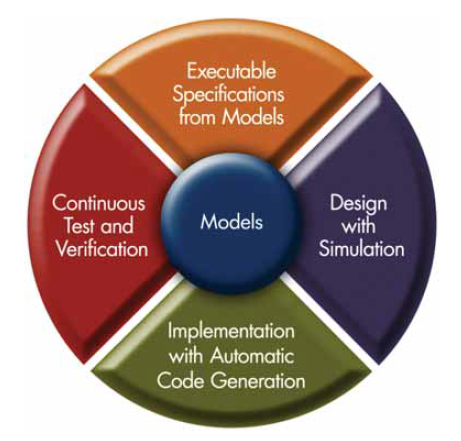
\includegraphics[width=.5\textwidth]{Figs/elementsMBD.PNG} 
     \caption{Elements of MBD from \citep{behboodian2006model}}
     \label{fig:elMBD} 
\end{figure} 

\subsection{Automatic Code Generation}

In classical development models the implementation phase follows the design, at this stage the developers will generate suitable software code in a selected language to implement the system. If the system definitions are not clear enough, the programmers would refer to system designer for clarification, but, despite these clarifications, there's still the possibility that the developed system may be different from the one that system designers had in mind. Even worse, it may contain coding errors that invalidates all the tests performed during the design. Although unlikely not even the case in which programmers job is perfect and there are no coding errors could make hand-coding the preferable approach, indeed just consider that there could be always the need to perform small changes inside the source code, such changes, whether not propagated in the models, rapidly will make the implementation divergent from the design. 
\paragraph{} MBD offers the capability to greatly improve the above approach. Within such methodology models can be used as the input to an automatic code generation tool. Usually MBD tools offers a framework at least for modeling and generate code from models, those framework commonly comprise a language offering the capability to explore model features and use them for producing target specific code.

%\paragraph{} Simulink, developed by \textit{The MathWorks Inc.}, is a block diagram environment for modeling, simulating and analyzing multidomain dynamic systems such as signal processing, control and communication applications. It supports system-level design, simulation, automatic code generation, and continuous test and verification of embedded systems. Thanks to its features, it is the \textit{de-facto} standard in MBD. 

\section{Hybrid Systems}

\subsection{State Machines}
\label{ssec:statemachines}

Systems are functions that transform signals. A broad class of systems can be characterized using the concept of state and the idea that
a system evolves through a sequence of changes in state, or state transitions. Such characterizations are called state-space models.
A state-space model describes a system procedurally, giving a sequence of step-by-step operations for the evolution of a system. It shows how the input signal drives changes in state, and how the output signal is produced. 
\paragraph{} A description of a system as a function involves three entities: the set of input signals, the set of output signals, and the function itself,
\begin{center}
$F: InputSignals \rightarrow OutputSignals $
\end{center}
For a state machine, the input and output signals have the form
\begin{center}
$EventFlow: \mathbb{N}_{0} \rightarrow Symbol$
\end{center}
where $\mathbb{N}_{0}=\{0,1,2,...\}$ and $Symbol$ is an arbitrary set. The domain of these signals represents an ordering relation that does not necessarily corresponds to time, discrete or continuous. Ordering of the domain means that it is possible to say whether one event occurs before or after another one, but without the knowledge of how much time elapses between these events.
\paragraph{} We can define \textit{state machine} that entity that constructs the output signal one symbol at a time by observing the input signal one symbol at a time. Specifically
\begin{center}
$StateMachine = (States, Inputs, Outputs, update, initialState)$
\end{center}
where $States$, $Inputs$, $Outputs$ are sets, $update$ is a function, and $initialState \in States$. The
meaning of these names is:
\begin{description}
	\item[States] is the set space
	\item[Inputs] is the input alphabet
    \item[Outputs] is the outputs alphabet
    \item[initialState] is the initial state $\in States$
    \item[update]: $States \times Inputs \rightarrow States \times Outputs$ is the update function
\end{description} 
The update function makes possible for the state machine to construct, step by step, the output signal by observing the input signal. In particular, if $x(n) \in States$ is the current state at step $n$, and $u(n) \in Inputs$ is the current input symbol, then current output symbol and the next state are given by the following
\begin{center}
$(x(n+1),y(n)) = update(x(n),u(n))$
\end{center}
The above could be decomposed in two different functions, one for new state and one for output 
\begin{flalign}
\label{form:nextstate}
&x(n+1)=nextstate(x(n),u(n)) \\
\label{form:output}
&y(n)=output(x(n),u(n))
\end{flalign}
where
\begin{flalign*}
&nextstate:  States \times Inputs \rightarrow States \\
&output:  States \times Inputs \rightarrow  Outputs
\end{flalign*}

\subsection{Time-Based Model}
\label{ssec:timemodel}

The previous section defines input and output signals of a state machine as a collection of \textit{events}. These events are generated in a domain which, usually, does not have a relation with a time set but, rather, represents just an ordered set. If we require events to happen at time instants that are multiple of a certain time quantity $\delta$ we have that
\begin{center}
$t\_e_{i}-t\_e_{j}=\alpha\cdot\delta,\quad i>j, \alpha \in \mathbb{Z}_{+}\quad \forall i,j \in \mathbb{N}_{0}$
\end{center}
where $t\_e_{i}$ and $t\_e_{j}$ are the time instant in which occur events $e_{i}$ and $e_{j}$. Under this assumption the state machine becomes a \textit{time-based model}, i.e. it reacts at all times in a base $T$.
\paragraph{} Another specialization of could be achieved by imposing, as further assumption, that state, input and output spaces be numeric sets
\begin{center}
$States=\mathbb{R}^{N},\quad Inputs=\mathbb{R}^{M},\quad Outputs=\mathbb{R}^{K}$
\end{center}
Combining the previous two assumptions we can define a \textit{discrete-time system}, and the index $n$ in (\ref{form:nextstate}) and (\ref{form:output}) is called \textit{time index}. Finally, we require that 
\begin{center}
$u(n) \in \mathbb{R}^{M}$ and $y(n) \in \mathbb{R}^{K} \quad \forall n \in T$
\end{center}
Therefore we disallow the capability, proper of state machines, to handle special "\textit{do nothing}" input called \textit{absent}. 

\subsection{LTI System}
\label{ssec:ltisys}

In discrete-time systems the time base $T \equiv \mathbb{Z}_{+}$, a definition of continuous-time system could be achieved if we relax $T$ to $\mathbb{R}_{0^{+}}$. This last category of systems shares many mathematical properties with its discrete-time version, but they can no longer be view as state machines since inputs, outputs, and state transitions do not occur at discrete instances.

\noindent
\\
Formally, a representation of a continuous time system is given, $\forall t \in \mathbb{R}_{0^{+}} $, by
\begin{flalign*}
&\dot{x}(t)=nextstate(x(t),u(t)) \\
&y(t)=output(x(t),u(t))
\end{flalign*}
The system is defined as \textit{linear} if functions $nextstate$ and $output$ are linear. It is also said \textit{time invariant} if both do not change over time. As result a system holding these two properties is said Linear Time Invariant (LTI). An interesting property of those system is that they can be represented in a compact matrix-based form. The $nextstate$ function is a $N\times (N+M)$ matrix, while the $output$ is a $K\times (N+M)$ matrix. If we partition both in two sub-matrix, the first of each comprising the first $N$ columns we get
\begin{flalign*}
\dot{x}(t)=Ax(t)+Bu(t) \\
y(t)=Cx(t)+Du(t)
\end{flalign*}
where $A \in \mathbb{R}^{N\times N}, B \in \mathbb{R}^{N\times M}, C \in \mathbb{R}^{K\times N}$ and $D \in \mathbb{R}^{K\times M}$.
\par The major difference between discrete and continuous system is that the new state is represented with the derivative of the current state instead of a function of current input and state. The motivation is that the derivative, which represents the trend of a function, better depicts the continuous evolution of the system rather than express it as a value at the successive time index.


\subsection{Mixed Models}

Sections \ref{ssec:statemachines} and \ref{ssec:timemodel} provided definitions of state machines and time-based model, trying to qualify the latter by imposing some constraint on the, more general, model of the first. In \ref{ssec:ltisys} such link was definitively broken due to the relaxation of the time to a continuous set. 
\paragraph{} In general, the two different models are used as alternative views of the same system. Even for simpler cases of discrete-time systems, which, though different from the continuous time, keep a precise mapping relationship between time and discrete time, retrieve the state machine relative to the time model is not straightforward. The reason is that operations of state machines normally acts according to a logic clear and understandable in response to situations or events that arise from the outside, such as pressing of buttons, the attainment of steady state conditions and so on.
\paragraph{} In order to get state machine models to coexist with time-based models, we need to interpret state transitions on the time line used for the time-based portion of the system, be it continuous time or discrete time. The resulting models are called hybrid systems. A hybrid system combines time-based signals with sequences of events. The time-
based signals are of the form $x : T \rightarrow R$ where $R$ is some range (such as $\mathbb{R}$ or $\mathbb{C}$), and $T$ is the time domain, discrete or continuous. In \ref{ssec:statemachines} we defined the event signals as 
\begin{center}
$u: \mathbb{N}_{0} \rightarrow Symbols$
\end{center}
for a hybrid system, however, these have to share a common time base with the time-based signals, so they must be in the form 
\begin{center}
$u: T \rightarrow Symbols$
\end{center} Thus, events occur in time. Typically, for most $t \in T$, $u(t) = absent$, meaning that the state machine does not perform any action.

\subsection{Formal Model}

The general structure of an hybrid system is shown in figure \ref{fig:hsstruct}.
\begin{figure}[!ht]
	\centering 
     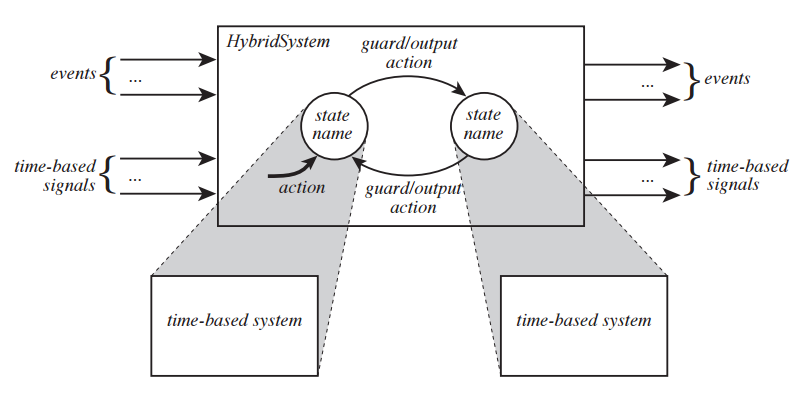
\includegraphics[width=\textwidth]{Figs/HS.PNG} 
     \caption{Hybrid System Structure} 
     \label{fig:hsstruct} 
\end{figure} 
\paragraph{} As previously mentioned, inputs and outputs may include either asynchronous events and time-based signals. In addition, each state of the state machine is associated with a time-based system, which is usually named \textit{refinement} of the state. The refinement represents the time-based behavior of the hybrid system while the internal machine is in the relative state. In order to prevent mess in the notation, those state referring to the state machine are usually called \textit{modes} while with \textit{states} are referred those of the refinements. Such notation strengthen the concept of a systems which alternates different time-based behaviors depending on the operating mode. Summarizing, for \textit{state} of an hybrid system is meant the pair $(m(t),s(t))$ where $s$ is the state of the time-based refinement system associated with mode $m$.

\noindent 
\\
A formal model for an hybrid system could be defined similarly to the one in \ref{ssec:statemachines}, indeed
\begin{center}
$HybridSystem = (States, Inputs, Outputs, TransitionStructure, initialState)$
\end{center}
where $States, Inputs$ and $Outputs$ are sets, $initialState \in States$ is the initial state and $TransitionStructure$ is the evolving law of the system in time $t \in T$, from now on we assume $T \equiv \mathbb{R}_{+}$.

\noindent
\\
$States = Modes \times RefinementStates$ represents the state space containing pairs \textit{mode}, \textit{refinementState} as previously mentioned. The set of possible modes is finite, while no constraint are on the refinement state set. 

\noindent
\\
$Inputs = InEvents \times TimeInputs$ corresponds to the set of input symbols. $InEvents$ is an alphabetic set in which each symbol stands for the description of the event, it also includes the special "do nothing" input \textit{absent}. $TimeInputs$, instead, contains all the inputs to which the refinement reacts. A complete input to the hybrid system is hence the functions pair $u:\mathbb{R}_{+}\rightarrow InEvents$ and $x:\mathbb{R}_{+}\rightarrow TimeInputs$. It's useful to recall that, apart for a limited number of cases, the function relative to the events for the most of the time is set to the value \textit{absent}.

\noindent
\\
$Outputs = OutEvents \times TimeOutputs$ is the set of output symbols. In strong analogy with what already done for the $Inputs$ set, we can identify $OutEvents$ as the alphabetic set containing those symbol representing the description of the event, and $TimeOutputs$ as the one containing all possible outputs for the refinement. The entire output of the hybrid system is then the functions pair $v:\mathbb{R}_{+}\rightarrow OutEvents$ and $y:\mathbb{R}_{+}\rightarrow TimeOutputs$. Even in this case for the most of the time the function $v(t)$ is equal to $absent$.

\noindent
\\
The $TransitionStructure$ determines how a mode transition occurs and how the refinement state changes over time. The evolution of an hybrid system occurs with the alternation of two phases, one associated to the transitioning and the other to the keeping of the current mode. In general, for state machines the transition between states is regulated by the verification of a particular conditions named \textit{guards}. Such conditions consists of an event,internal or external, occurrence. For hybrid system the concept of guard is slightly extended, in particular, given the system in a mode $m$ with relative refinement in the state $s$, the guard leading to a destination mode $d$ has the form
\begin{center}
$G_{m,d}=U_{m,d} \times X_{m,d} \times S_{m,d} \subset InEvents \times TimeInputs \times RefinementStates$
\end{center}
commonly, associated to a mode transition there is an output event $v_{m,d}$ and a function \textit{action}, $A_{m,d}:RefinementStates\rightarrow RefinementStates$, which updates the value of the refinement state. The transition from mode $m$ to mode $d$ occurs at time $t$ if the triple $(u(t),x(t),s(t))\in G_{m,d}$. If it is the case, after the transition (which is considered instantaneous) the system starts operating in mode $d$ with refinement state equal to $s(t+) = A_{m,d}(s(t))$, producing the output event $v_{m,d}$. In the case no guard is satisfied at time $t$ the systems evolves in the current mode. The refinement state $s(t)$ and the time-based output $y(t)$ are then determined by the time-based input signal $x(t)$ according to equations governing
the refinement dynamics (see Sec.\ref{ssec:ltisys}). The alternation of the two phases discussed above can be represented as $\bigcup\limits_{i=0}^{\infty}(t_i,t_{i+1}]$, during each interval the active phase is the one who maintain constant the operation mode, while the transition phase take place at the rightmost time instant of every interval.

\subsection{Examples}

\paragraph{Timed Automata} The simplest continuous-time hybrid systems that can be analyzed is a timed finite state machine measuring passage of time, it has a very simple refinement dynamics that can be modeled with a first-order differential equation,
\begin{align*}
\dot{s}(t)=1, \quad \forall t \in T_m
\end{align*}
where $T_m \subset T$ is the subset of time during which the hybrid system is in mode $m$. Figure \ref{fig:tickgen} shows a timed automata which generates a tick at time intervals alternating between 1 and 2 seconds. Although simple such example shows all the basic features of an hybrid system, namely the alternate evolution between time-count phase and tick-phase (Fig.\ref{fig:tickgenmode}), output event signal most of the time at absent value (Fig.\ref{fig:tickgenout}) and refinement output, equal to the state in this case, as a signal resulting from a differential equation (Fig.\ref{fig:tickgenstate}).
\begin{figure}[!ht]
	\centering 
     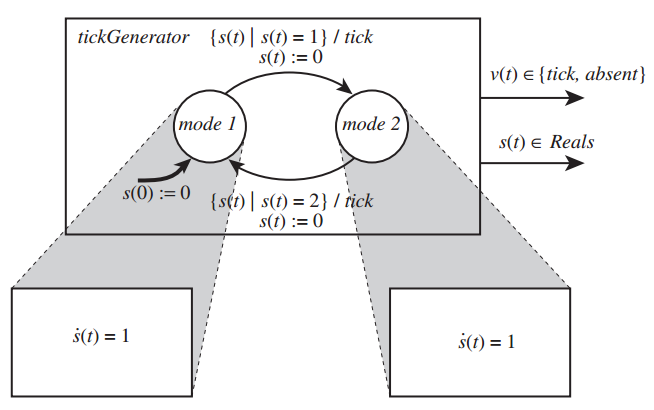
\includegraphics[width=.7\textwidth]{Figs/tickgen.PNG} 
     \caption{Hybrid System: Tick Generator} 
     \label{fig:tickgen} 
\end{figure}

\begin{figure}[!h]
  \centering
  \begin{subfigure}[b]{0.3\textwidth}
    \centering
    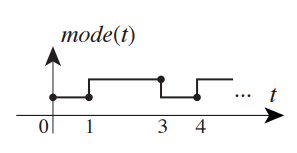
\includegraphics[width=\textwidth]{Figs/tickgenmode.PNG}
    \caption{Mode}
    \label{fig:tickgenmode}
  \end{subfigure}
  \begin{subfigure}[b]{0.3\textwidth}
    \centering
    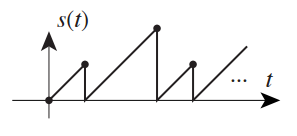
\includegraphics[width=\textwidth]{Figs/tickgenstate.PNG}
    \caption{Refinement Out}
    \label{fig:tickgenstate}
  \end{subfigure}
  \begin{subfigure}[b]{0.3\textwidth}
    \centering
    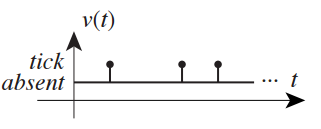
\includegraphics[width=\textwidth]{Figs/tickgenout.PNG}
    \caption{Out Event}
    \label{fig:tickgenout}
  \end{subfigure}
  \caption{Tick Generator Internals}
\end{figure}

\paragraph{Bouncing Ball} An more interesting example is an hybrid system describing the dynamics of a bouncing ball. In this case the adoption of a mixed model greatly simplifies the representation of such a system, since, being it non-linear, finding a representation only through differential equation is not easy.
\par At time $t=0$ the ball is dropped from a certain height $y(0)=h$, it freely falls, with constant velocity $\dot{y}(t) < 0\: m/s$, up to hit the ground, say at time $t1$. In that instant the \textit{bounce} events occurs and, under the assumption of inelastic collision, the ball bounces back with an inverted velocity $-a \dot{y}(t1)$, where $a \in (0,1)$. After the ball reaches a certain height it falls back  repeatedly. The model of the bouncing ball is illustrated in Figure \ref{fig:bounballhs}

\begin{figure}[!ht]
	\centering 
    \begin{subfigure}[b]{0.45\textwidth}
    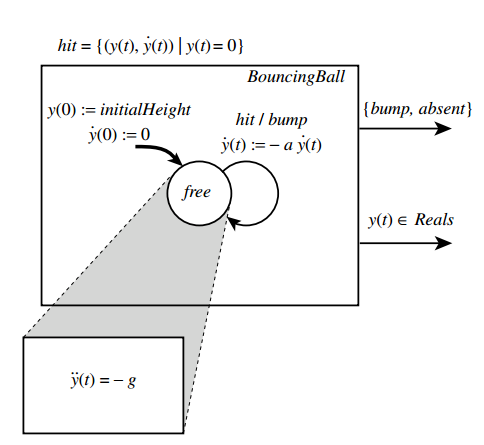
\includegraphics[width=\textwidth]{Figs/bounball.png} 
    	\caption{hybrid system} 
        \label{fig:bounballhs}
    \end{subfigure}
    \begin{subfigure}[b]{0.45\textwidth}
    	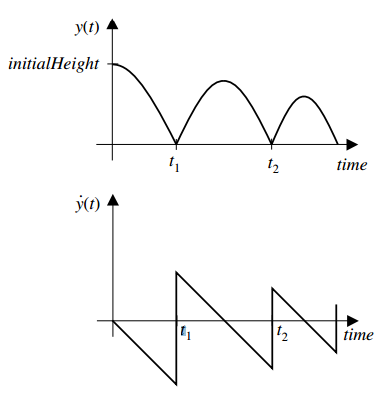
\includegraphics[width=\textwidth]{Figs/bounballout.png} 
        \caption{height and velocity} 
    	\label{fig:bounballout}
    \end{subfigure}    
     \caption{Hybrid System: Bouncing Ball} 
     \label{fig:bounball} 
\end{figure}

The \textit{hit} condition is raised whenever the height of the ball is equal to 0, namely whenever it reaches the ground. In all other time instants in order to get position and velocity of the ball is enough to double integrate the acceleration (Fig.\ref{fig:bounballout}).
\chapter{Formal Verification}

\section{Temporal Logic}
Temporal logic is a rigorous formalism for specifying behaviors of continuous and discrete systems \citep{pnueli1992temporal,manna2012temporal}
provides simple constructs to describe the order in which different “events” in the system
should happen. The basic infrastructure of a formal language provides syntactical operators to handle property verification during time. In literature plenty of formalisms have been proposed, each one specializing either time or application specific features. First part of this chapter aims to analyze some of them starting from their common ancestor, providing also a general comparison.

\subsection{Linear Temporal Logic}
\label{ssec:LTL}

In the Linear Temporal Logic (LTL) time is implicitly represented as an enumerated sequence of reaction steps occurring in a discrete time space. Such temporal logics was developed to check properties in (typically hardware) systems with boolean, discrete-time signals. 
\par LTL with \textit{future} and \textit{past} is defined using the following
syntax:
\begin{center}
$\varphi := \quad p \quad | \quad \neg \varphi \quad | \quad \varphi \vee \varphi \quad | \quad \ocircle  \varphi \quad | \quad \circleddash \varphi \quad | \quad \varphi \; \EuScript{U} \; \varphi |  \quad \varphi \; \EuScript{S} \; \varphi $
\end{center}
where $p$ belongs to a set $P = \{ p_1,\dots,p_n \}$ of propositions indicating values of the corresponding state variable. LTL is interpreted over n-dimensional Boolean $\omega$-sequences of the form $\omega : \mathbb{N} \rightarrow \mathbb{B}^n$. We use $\omega[t]$ to denote the value of a sequence $\omega$ at position $t$ and abuse $p$ to denote the projection of $w$ on variable $p$. The basic future temporal operators are \textit{next} ($\ocircle$), which specifies what should hold in the next step and \textit{until} ($\EuScript{U}$), which requires $\varphi_1$ to hold until $\varphi_2$ becomes true, without bounding the temporal distance to this becoming. From these basic LTL operators one can derive other standard Boolean operators as well as temporal operators such as \textit{eventually} ($\lozenge$) and \textit{always} ($\Box$): 
\begin{center}
$\lozenge \varphi = True \;\; \EuScript{U} \;\; \varphi\quad$and$\quad \Box \varphi = \neg \lozenge \neg \varphi$
\end{center}
Analogously, by means the past temporal operators, is possible to define \textit{eventually in the past}($\mathrlap{\lozenge}{-}$) and \textit{always in the past}($\mathrlap{\Box}{-}$)
\begin{center}
$\mathrlap{\lozenge}{-} \varphi =  True \;\; \EuScript{S}  \;\; \varphi\quad$and$\quad\mathrlap{\Box}{-} \varphi = \neg \mathrlap{\lozenge}{-} \neg \varphi$
\end{center}

The satisfaction relation $(\omega, t) \models \varphi$ indicating that a sequence $\omega$ satisfies $\varphi$ starting from position $t$, is defined inductively as follows:
\begin{equation}
\label{form:LTLop}
\begin{aligned}
 p   & & &(\omega, t) \models \varphi & & &\leftrightarrow & & &p[t] = 1 \\
 not \; \varphi & & &(\omega, t) \models \neg \varphi  & & &\leftrightarrow  & & &(\omega, t) \nvDash \varphi \\
 \varphi_1 \; or \; \varphi_2 & & &(\omega, t) \models \varphi_1 \vee \varphi_2  & & &\leftrightarrow  & & &(\omega, t) \models \varphi_1 \; or \; (\omega, t) \models \varphi_2 \\
 next \; \varphi & & &(\omega, t) \models \ocircle \varphi  & & &\leftrightarrow  & & &(\omega, t+1) \models \varphi \\
 previously \; \varphi & & &(\omega, t) \models \circleddash \varphi  & & &\leftrightarrow  & & &(\omega, t-1) \models \varphi \\
 \varphi_1 \; until \; \varphi_2 & & &(\omega, t) \models \varphi_1 \EuScript{U} \varphi_2  & & &\leftrightarrow  & & & \exists \; t^\prime \in [t, \infty) \; (\omega, t^\prime) \models \varphi_1 \; and \; \forall \; t^{\prime \prime} \in [t, t^\prime), (\omega, t^{\prime \prime}) \models \varphi_2\\
 \varphi_1 \; since \; \varphi_2 & & &(\omega, t) \models \varphi_1 \EuScript{S} \varphi_2  & & &\leftrightarrow  & & & \exists \; t^\prime \in [0, t] \; (\omega, t^\prime) \models \varphi_1 \; and \; \forall \; t^{\prime \prime} \in (t^\prime, t], (\omega, t^{\prime\prime}) \models \varphi_2\\
 \\
 eventually \; \varphi & & &(\omega, t) \models \lozenge \varphi  & & &\leftrightarrow  & & & \exists \; t^\prime \ge t \; (\omega, t^\prime) \models \varphi \\
 always \; \varphi & & &(\omega, t) \models \Box \varphi  & & &\leftrightarrow  & & & \forall \; t^\prime \ge t \; (\omega, t^\prime) \models \varphi
\end{aligned}
\end{equation}

A major difficulty in checking properties expressed in future LTL is due to the \textit{non-causal} definition of the satisfaction relation. In other words, the satisfiability of $\varphi$ at time $t$ may depend on the value of $\omega$ at some future time instant $t^\prime \geq t$. Even worse, some temporal operators refer to future time instants in a \textit{quantified} manner, for example, requiring some $p$ to hold in all future time instants. The satisfiability of such a property may sometime be determined only at infinity, that is, “after” we can be sure
that no instance of $\neg p$ is observed.
\par The causality problem is not present anymore when the recursion goes backward in time, meaning that the satisfaction of a past formula $\varphi$ by a sequence $\omega$ at position $t$ is determined only according to the values of $\omega$ at the interval $[0, t]$. However the futuristic specification keeps a style more natural for humans, for this reason it has been adopted also by industrial specification languages such as PSL (\ref{sec:PSL}).

\paragraph{Evaluation over incomplete behavior}

Monitors do not exploit features of the model representing the system $S$, but rather observe sequences, i.e. model's outputs, as they are produced during simulation. Although the LTL semantic is defined over \textit{complete infinite sequences}, that is for all possible behaviors, is not possible to observe infinite sequence in finite time. Hence, trying to extend the LTL semantic to \textit{incomplete behaviors} represents the hardest challenge in monitoring.
\par At the end of the observation of a certain sequence $\omega$ we can assert one of the following with respect to the property $\varphi$
\begin{enumerate}
\item \textit{$\omega$ satisfies $\varphi$.} Such situation happens, for example, when $\varphi=\lozenge p$ and $p$ occurs in $\omega$.
\item \textit{$\omega$ not satisfies $\varphi$.} For example, when $\varphi=\Box \neg p$ and $p$ occurs in $\omega$.
\item \textit{$\omega$ is undecided.} For example, when $\varphi=\lozenge p$ and $p$ has not yet occurred in $\omega$.
\end{enumerate}
The category "undecided" can be further refined in order to distinguish, for instance, the "not yet violated" ($\varphi=\Box \neg p$) category from the "not yet satisfied" one ($\varphi=\lozenge p$).\\
Even for those cases in which the satisfiability of a property cannot be determined from the observed behavior we would like to give an answer at the end of the sequence. In order to achieve such objective we may consider some LTL sub-classes. One is the bounded-LTL. It provides only \textit{next} as temporal operator, which, in turn, can be used to derive others such as bounded-always and bounded-eventually
\begin{center}
$ \Box_{[0,r]}\varphi = \bigwedge  \limits_{i=0}^{r-1} \ocircle^i \varphi\;\;$ and $\;\;\lozenge_{[0,r]}\varphi = \bigvee  \limits_{i=0}^{r-1} \ocircle^i \varphi$
\end{center}
where $\ocircle^i$ is a shorthand for $\ocircle(\ocircle(\dots\ocircle)p\dots))$. Within this context of timed formulas a global property that has not been violated during the formula's lifetime is considered satisfied. Analogously a property expressing an eventuality not observed during the formula's lifetime is considered violated.

\subsection{Computation Tree Logic}

LTL formulas define properties referring individual executions, or simulations, that is, operators are provided for describing events along a single computation path. 
\par The Computation Tree Logic (CTL) \citep{clarke2008design} extends this concept by expressing formulas with respect to many executions, or simulations, at once. In this sense it belongs to the family of  \textit{branching time logic}, in which operators quantify over the paths that are possible from a given state. The main feature provided by logic such as CTL is the possibility to add temporal connectives to the usual the usual atomic propositional logic formulas.  The temporal connectives are expressions about paths into the future that the state of the system can follow.
\paragraph{} The occurrence of a CTL formula is specified by means the pair \textit{path}, \textit{temporal} quantifiers. The first regards the possible execution paths that the system can follow starting from the current one. The second, instead, relates the occurrences within each single path. 
\par It's clear how LTL logic represents a subset of CTL, in fact an LTL formula can be view as a CTL formula without the specification of the branch quantifier. However, part of the literature uses identify with CTL the sub-logic related to path and with CTL$^*$ the one which unifies both path and temporal quantifiers. According that, LTL and CTL becomes two intersecting set, while CTL$^*$ is the superset containing both. Anyway, for the sake of simplicity, in what follows we will make no difference between CTL and CTL$^*$, using the first in place of the second.

\paragraph{} When evaluating a CTL formula the first member to be considered is the path quantifier. It can be
\begin{description}
\item[A] meaning on \textit{all} the path from the current state, read as "\textit{inevitably}"
\item[E] meaning on \textit{at least one} path from the current state, read as "\textit{possibly}"
\end{description}
Once defined the occurrence among the paths, the second member to consider is the temporal quantifier, i.e.
\begin{description}
\item[X] meaning the next state
\item[G] meaning all the future states, read as "\textit{globally}".
\item[F] meaning in some future state
\item[U] meaning until
\end{description}
Combining the previous operators is possible to generate different types of formulas, suppose that the system is in some state $S$ the formula
\begin{description}
\item[$\varphi$] is true iff it is satisfied by the current state $S$
\item[AX($\varphi$)] is true iff $\varphi$ is true for every immediate successor of state $S$
\item[AG($\varphi$)] is true iff $\varphi$ is true for every successor to state $S$, including $S$. That is, $\varphi$ is true for all states on all paths into the future from $S$, i.e. the subtree originating from $S$
\item[AF($\varphi$)] is true iff on all paths into the future from $S$, there is a state where $\varphi$ holds
\item[A [$\varphi_1$ U $\varphi_2$]] is true iff all paths starting in state $S$ satisfy $\varphi_1$ until the reach a state in which $\varphi_2$ holds
\\
\item[EX($\varphi$)] is true iff $\varphi$ is true for at least one immediate successor to state $S$
\item[EG($\varphi$)]  if true iff there is a path from $S$ into the future for which $\varphi$ holds for every state on the path, including $S$
\item[EF($\varphi$)] is true iff there exists a path into the future from $S$ on which there is a state where $\varphi$ holds
\item[E [$\varphi_1$ U $\varphi_2$]] is true iff there exists a path starting in state $S$ that satisfies $\varphi_1$ until reaching a state in which $\varphi_2$ holds
\end{description}
A graphical representation of the above formulas is shown in Figure \ref{fig:ctl}
\begin{figure}[!h]
	\centering 
     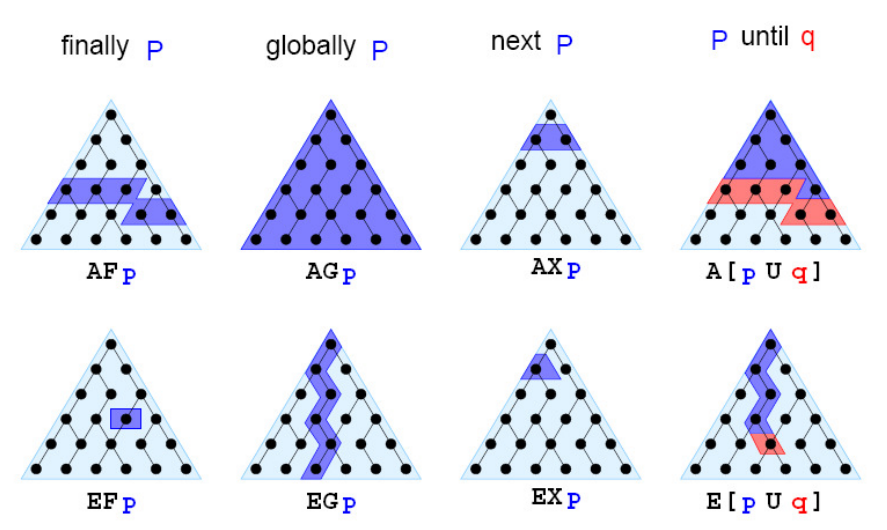
\includegraphics[width=.9\textwidth]{Figs/ctl.PNG} 
     \caption{CTL formulas} 
     \label{fig:ctl} 
\end{figure} 

\noindent
A subset Computation Tree Logic is supported for verification in UPPAAL, which is an integrated tool environment for modeling, validation and verification of real-time systems modeled as networks of timed automata \citep{uppaal}.

\subsection{Property Specification Language}
\label{sec:PSL}

The Property Specification Language (PSL) \citep{eisner2007practical} is a formal language for specification of electronic system behavior, compatible with multiple electronic system design languages. In 2005 it became an IEEE standard \citep{ieee2005ieee}. PSL was designed to be mathematically rigorous, with the result that a PSL specification is both precise and automatically verifiable. Thus, a hardware specification written in PSL is machine readable and can be used as input to verification tools.

\paragraph{} Being a specification language whose targets is the hardware, signals in PSL are used as stream of bits having a fixed length, and , for the same reason, time is meant as a sequences of \textit{clock-cycles}. The structure of PSL is based on four layers
\begin{enumerate}[label={--}]
\item The \textit{boolean layer} is composed of Boolean expressions. PSL interprets a high signal as true, and a low signal as false, independent of whether the signal is active-high or active-low. Operations of the Boolean layer are expressed through the supported hardware specification languages such as Verilog, VHDL and so on.
\item The \textit{temporal layer} consists of temporal properties which describe the relationships between Boolean expressions over time. The semantic of temporal operators is quite similar to the LTL ones.
\item The \textit{verification layer} consists of directives which describe how the temporal properties should be used by verification tools. For instance, is possible to define verification or assumption directives, which tells the tools to verify the value of some property or specify coverage criteria. The verification layer also provides a means to group PSL statements into \textit{verification units}.
\item The \textit{modeling layer} provides a means to model behavior of design inputs, and to declare and give behavior to auxiliary signals and variables
\end{enumerate}

While the Boolean layer consists of Boolean expressions that hold or do not hold at a given cycle, the temporal layer provides a way to describe relationships between Boolean expressions over time. A PSL assertion typically looks in only one direction – forwards from the first cycle. Thus, the simplest PSL assertion \textbf{assert a;} states that signal \textbf{a} should hold at the very first cycle. 
\noindent
\\
The PSL temporal operators are the following
\begin{description}
\item[always ($p$)] meaning that property $p$ must \textit{globally} hold
\item[never ($p$)] meaning that property $p$ must \textit{never} hold
\item[next ($p$)] will hold if its operand, $p$, holds at the next clock-cycle. Variations on the next operator allows to specify ranges of future cycles, i.e. a  \textbf{next a[i:j]($p$)} property holds if its operand holds in all of the cycles from the $i^{th}$ next cycle through the $j^{th}$ next cycle, inclusive.
\item[$p$ until $q$] provides a way to move forward, meaning that property $p$ must hold \textit{until} $q$ hold. In order to include the cycle in which $q$ holds the \textbf{until\_} is normally used.
\item[$p$ before $q$] is dual to \textbf{until} and requires that its first operand happen strictly before
its second. Even for this case in order to include the cycle in which $q$ holds, namely is allowed an overlap between left and right sides, the \textbf{before\_} is used.
\item[eventually!($p$)] allows you to specify that $p$ must occur in the future without saying exactly when.
\end{description}
A good feature of PSL is that it let user choose how the formulas are evaluated in cases of incomplete behavior. Such problem, already discussed in section \ref{ssec:LTL}, rises whenever the simulation, or execution, time is not enough to determine the satisfiability of a formula. PSL handles this providing the possibility to define the strength of an operator, therefore operators can be claimed as \textit{strong}  or \textit{weak} depending on the addition of an exclamation mark (\textbf{!}) to their names. Formulas with strong operators, marked with (\textbf{!}), are considered satisfied if the simulation time is \textit{enough}  and the property holds, for instance \textbf{next![n]} indicate that at least $n$ cycles are needed. Some operators, anyway ,constitutes an exception since they are only allowed in their weak (\textbf{always}, \textbf{never}) or strong (\textbf{eventually!}) versions. Moreover, PSL offers many other versions of \textbf{next} associated with occurrence of events rather than cycles, for further details refer \citep{eisner2007practical}.

\subsection{Signal Temporal Logic}
\label{sec:STL}

Signal Temporal Logic (STL) \citep{maler2004monitoring} is a temporal logic for specifying properties on \textit{dense-time real-valued signals}. Such a logic is particularly useful in domains like \textit{control systems}, where continuous variables are used to model the physical plant	under control. The natural models for such systems are differential equations, for purely continuous systems, or hybrid systems when the dynamics is mixed and contains mode switching, saturation, etc. Before going into details of STL is useful to analyze it's direct ancestor MITL.

\paragraph{Metric Interval Temporal Logic} The \textit{real-time temporal logic} MITL \citep{alur1996benefits} allows reasoning over Boolean signals over dense-time domains. Formally, signals are functions of the form $s: \mathbb{T} \rightarrow \mathbb{B}$, where the time domain $\mathbb{T}$ is the set of non-negative real numbers $\mathbb{R}_+$.
\par We consider the logic MITL$_{[a,b]}$ as a fragment of MITL, such that all temporal modalities are restricted to intervals of the form [$a, b$] with $0 \leq a < b$ and $a, b \in \mathbb{Q}+$. Similarly to \ref{ssec:LTL}, the use of bounded temporal properties is justified by the nature of monitoring where the behavior of a system is observed for a finite time interval. The basic formulas of MITL$_{[a,b]}$ are defined by the grammar
\begin{center}
$\varphi := \quad p \quad | \quad \neg \varphi \quad | \quad \varphi \vee \varphi \quad | \quad \varphi_1 \; \EuScript{U}_{[a,b]} \; \varphi_2 $
\end{center}
From basic MITL[a,b] operators one can derive other standard Boolean and temporal operators, in particular the time-constrained eventually and always operators:
\begin{align*}
\lozenge_{[a,b]} \varphi &= True \; \EuScript{U}_{[a,b]} \; \varphi \\
\Box_{[a,b]} \varphi &= \neg \lozenge_{[a,b]} \neg \varphi 
\end{align*}
The semantic of the unbounded operators is equivalent to the one provided for LTL (\ref{form:LTLop}), while the introduction of the time window modifies \textit{until}, \textit{eventually} and \textit{always} as follow
\begin{align*}
(s, t) \models \varphi_1 \EuScript{U}_{[a,b]} \varphi_2 &\leftrightarrow \exists \; t^\prime \in [t+a, t+b] \; (s, t^\prime) \models \varphi_2 \; and \; \forall \; t^{\prime \prime} \in [t, t^\prime], (s, t^{\prime \prime}) \models \varphi_1 \\
(s, t) \models \lozenge_{[a,b]} \varphi &\leftrightarrow \exists \; t^\prime \in [t+a, t+b], (s, t^\prime) \models \varphi \\
(s, t) \models \Box_{[a,b]} \varphi &\leftrightarrow \forall \; t^\prime \in [t+a, t+b], (s, t^\prime) \models \varphi
\end{align*}
By using bounded operators we avoid the problems related to the ambiguity
of $\models$ when applied to finite signals or sequences. Nevertheless, even for MITL$_{[a,b]}$ certain signals are too short to determine satisfaction of the formula, for example the property $\Box_{[a,b]}\lozenge_{[c,d]}p$ cannot be evaluated on signals shorter than $b + d$.

\paragraph{} We can now extend our semantic domain and logic to real-valued signals. While Boolean signals of finite variability admit a finite representation, this is typically not the case for real-valued signals which are often represented via sampling, that is a sequence
of time stamped values of the form $(t, s[t])$. Although the semantics of the logic is defined in terms of the mathematical objects, for signals of the from $s : \mathbb{T} \rightarrow \mathbb{R}^n$ is not possible to ignore issues related to their effective representation based on the output of some numerical simulator. For this reason STL does not directly cope with continuous signal, but rather via a set of abstraction of the form $\mu : \mathbb{R}^n \rightarrow \mathbb{B}$. Typically $\mu$ partitions the continuous state-space according to the satisfaction of some inequality constraints on the real variables. As long as $\mu(s[t])$ remains constant we do not really care about the exact value of $s[t]$. However, in order to evaluate formulas we need the sampling to be sufficiently dense so that all such transitions can be detected when they happen. From now on we assume that we deal with signals that are well-behaving with respect to every $\mu$, that is, every change in $\mu(s)$ is detected in the sense that every point $t$ such that $\displaystyle{\mu(s[t]) \neq \; \lim_{t^\prime\to t} \; \mu(s[t]^\prime)}$ is included in the sampling.

\paragraph{} We can define an STL formula as a MITL$_{[a,b]}$ formula over the atomic propositions $\mu_1(s(t)),\dots,\mu_m(s(t))$, where each $\mu_i$ is a predicate of the form $\mu_i:\mathbb{R}^n\rightarrow\mathbb{B}$. The monitoring process for STL formula decomposes hence into two phases, in which the first is always the construction of a Boolean “filter” for every $\mu_i \in U = \{\mu_1 , \dots ,\mu_m \}$, which transforms $s$ into a Boolean signal $p_i = \mu_i(s)$.

\subsection{Summary}

\section{Patterns Identification}

The drawback to using temporal logics for property specification is their steep learning curve for industrial practitioners. Consequently, designers and developers will be less likely to use verification tools if they must devote large amounts of time to learning a specification language. Even with significant expertise, dealing with the complexity of such a specification could be daunting. As many other disciplines, like \textit{software engineering}, complexity in this context is addressed through the definition and use of common \textit{patterns}. Patterns are meant as a further levels of abstraction, parameterizable and often formalism-independent. 

\subsection{Property Specification Patterns}

Property specification patterns \citep{dwyer1998property} describe commonly observed requirements in a generalized manner. Observing the several formalisms introduced before is possible to notice how there are two basic parts of properties that commonly occur. The first tells when the property should hold, and the second tells what condition should be satisfied during this time. Precisely each formula consists of two pieces: a \textit{scope} and a \textit{pattern}. The scopes defines \textit{when} a particular property should hold during the simulation, the pattern, instead, the condition that must be satisfied. The are five basic kinds of scopes that can be recognized,
\begin{description}
\item[Globally] meaning the entire simulation
\item[Before R] meaning the entire execution up to the occurrence of \textbf{R}
\item[After Q] meaning the entire execution from the occurrence of \textbf{Q}
\item[Between Q and R] any piece of simulation from the occurrence of Q and the occurrence of \textbf{R}
\item[After Q until R] like above but holds even if \textbf{R} does not occur
\end{description}
\begin{figure}[!h]
	\centering 
     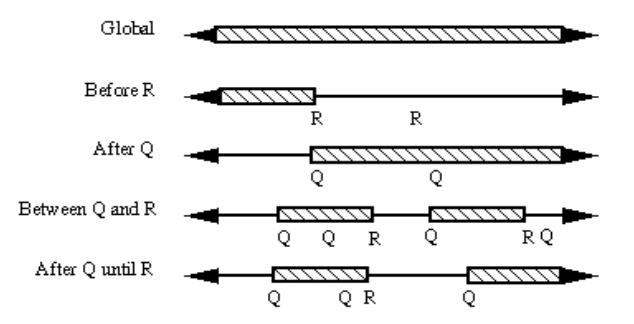
\includegraphics[width=.7\textwidth]{Figs/scopes.PNG} 
     \caption{Property Scopes} 
     \label{fig:scopes} 
\end{figure} 
Figure \ref{fig:scopes} illustrates the portions of an execution that are designed by the different kind of scopes.
\par Patterns are organized in a hierarchical manner based on their semantic. A the first level they are divided by \textit{occurrence} and \textit{order}. Firsts are used to express requirements related to the existence (or lack of existence) of certain states/events during well-defined regions of system execution, while seconds are used to express requirements related to pairs of states/events during well-defined regions of system execution. For both categories regions are defined using \textit{scopes}. In the class of Occurrence patterns we find
\begin{description}
\item[$P$ is false (Absence)] to describe a portion of a system's execution that is free of certain events or states.
\item[$P$ is true (Universality)] to describe a portion of a system's execution which contains only states that have a desired property.
\item[$P$ becomes true (Existence)] to describe a portion of a system's execution that contains an instance of certain events or states.
\item[$P$ occur at most $N$ times (Bounded Existence)] to describe a portion of a system's execution that contains at most a specified number of instances of a designated state transition or event.
\end{description}
while Order patterns are
\begin{description}
\item[$S$ precedes $P$ (Precedence)] to describe relationships between a pair of events/states where the occurrence of the first is a necessary pre-condition for an occurrence of the second.
\item[$S$ responds to $P$ (Response)] to describe cause-effect relationships between a pair of events/states.
\item[$Q_1\dots Q_n$ precedes $P_1\dots P_n$ (Precedence Chain)] to describe a relationship between a sequence of events/states and a sequence of events/states. The occurrence of sequence $P_1\dots P_n$ must be preceded by an occurrence of the the sequence $Q_1\dots Q_n$.
\item[$P_1\dots P_n$ responds $Q_1\dots Q_n$ (Response chain)] to describe a relationship between stimulus events and a sequence of response events. The occurrence of the stimulus $P_1\dots P_n$ must be followed by an occurrence of the sequence $Q_1\dots Q_n$.
\end{description}
Clearly patterns are not unique in the sense that one can be achieved by combination of some others. The Absence, for instance, is dual to Existence, while Precedence is converse to Response. This redundancy does not represents an issue but rather extends the usability of those patterns even in formalisms that not provide complete support for all scope operators. Figure \ref{fig:phierarchy} provides an overview of patterns classification.
\begin{figure}[!h]
	\centering 
     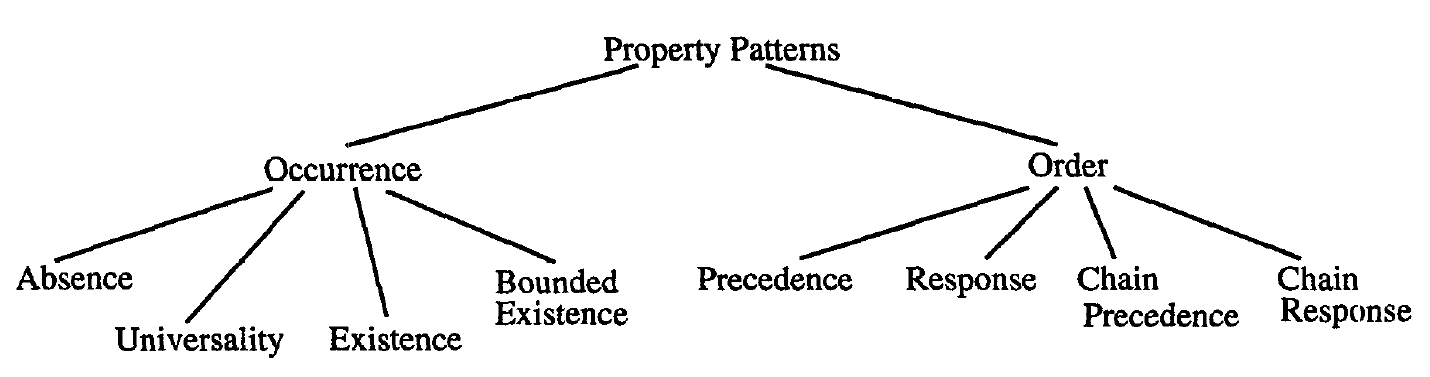
\includegraphics[width=.9\textwidth]{Figs/hierarchy.PNG} 
     \caption{Pattern Hierarchy} 
     \label{fig:phierarchy} 
\end{figure} 

Being each pattern defined over a scope, the number of possible achievable combinations corresponds to the dimension of the set generated by the product of scope and pattern sets. Each combination could be mapped in a specific requirements, therefore it can be independently translated in a chosen formalism. For the sake of briefness we show the complete LTL an CTL formalization for just a pattern, and refer \citep{specpatterns} for an exhaustive list. 
\par Before describe the pattern lets define the \textit{weak until} operator $\EuScript{W}$ which is used make less verbose the expression of some formulas.
\begin{center}
\begin{tabular}{ll}
LTL: &$P \;\EuScript{W}\; Q = P \;\EuScript{U} \; (Q\; |\; \Box\:P) $ \\
CTL: &$P$ \textbf{W} $Q = \neg$E ($\neg Q$ \textbf{U} ($\neg P$ $\&$ $\neg Q$))
\end{tabular}
\end{center}
\paragraph{Universality} \textbf{$P$ is true}\noindent\\
\begin{tabular}{ll}
\textit{Scope} & \textit{LTL} \\
Globally & $ \Box\;P$ \\ 
Before $R$ & $A\;R\rightarrow(P\;\EuScript{U}\;R)$\\
  After $Q$ & $ \Box\;R\rightarrow(Q\rightarrow \Box\; P)$	\\
Between $R$ and $Q$ & $ \Box\;((Q\; \&\; \neg R\; \&\; \lozenge\:R)\rightarrow(P\;\EuScript{U}\;R))$	\\
\end{tabular}
\\
\\
\begin{tabular}{ll}
\textit{Scope} & \textit{CTL} \\
Globally & \textbf{AG}($P$) \\ 
Before $R$ & \textbf{A}(($P$ | \textbf{AG}($\neg R$)) \textbf{W} $R$)\\
After $Q$ & \textbf{AG}($Q \rightarrow $ \textbf{AG}($P$))	\\
Between $R$ and $Q$ & \textbf{AG}($Q\;\&\;\neg R \rightarrow$ \textbf{A}(($P$ | \textbf{AG}($\neg R$)) \textbf{W} $R$	\\
After $Q$ unitl $R$ & \textbf{AG}($Q\;\&\;\neg R \rightarrow$ \textbf{A}($P$ \textbf{W} $R$))
\end{tabular}

\subsection{Domain Patterns}
\label{ssec:dompatterns}

When dealing with complex systems quite often the requirements analysis is performed at different levels of abstraction. As result the complete specification is provided by many requirements documents, in which requirements of a certain level are grouped according to derivation from a \textit{parent requirement} belonging to an higher level. 
\par A typical scenario for control systems is that high-level requirements focus all those properties specific of that application domain. Examples are the so called \textit{performance requirements}, which assess features of the system response over time. Since they refer properties having a well-known mathematical representation such kind of requirements in turn are prone to have a parameterizable definition. In other words they are suitable to become domain specific patterns.
\par Two typical performance requirements expressed in natural language are the following
\begin{quote}
\begin{enumerate}
\label{en:ptreq}
\item \textit{The Driver System (DRV) shall accelerate the motor from zero to $x_1$ rpm in less than $t_1$ sec, with an overshoot of less than $x_2$ rpm  and a time to settle to within $\pm x_3$ rpm of $x_4$ rpm of less than $t_2$ ms with a system inertia less than or equal to $S_{In}$}
\item \textit{The Driver System (DRV) shall decelerate the motor from $x_1$ to zero rpm in less than $t_1$ sec, with an undershoot of less than $x_2$ rpm and a time to settle to within $\pm x_3$ rpm of  zero rpm of less than $t_2$ ms with a system inertia less than or equal to $S_{In}$}
\end{enumerate}
\end{quote} 
An informal definition of the addressed requirements is the following
\begin{description}
\item[Rise(Fall)-time] is the amount of time it takes for a signal to rise (fall) from an initial value to another value some distance from an expected steady state value in response to a step input  (Fig.\ref{fig:risetime})
\item[Overshoot (Undershoot)] is a quantity that defines how much a signal goes beyond an expected steady state value in response to a step input (Fig.\ref{fig:overshoot})
\item[Settling-Time] is the time it takes a signal to reach and remain within a band around a steady state value in response to a step input (Fig.\ref{fig:settime})
\end{description}
\begin{figure}[h]
    \centering
    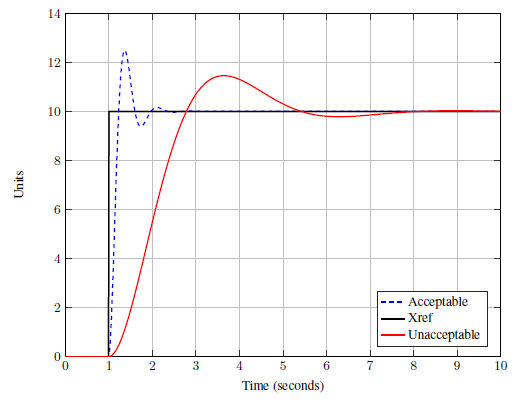
\includegraphics[width=.6\textwidth]{Figs/risetime.PNG}
    \caption{Rise Time}
    \label{fig:risetime}
\end{figure}
\begin{figure}[h]
    \centering
    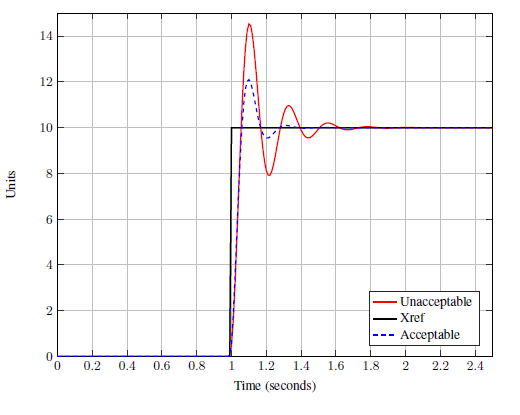
\includegraphics[width=.6\textwidth]{Figs/overshoot.PNG}
    \caption{Overshoot}
    \label{fig:overshoot}
\end{figure}
\begin{figure}[ht]
    \centering
    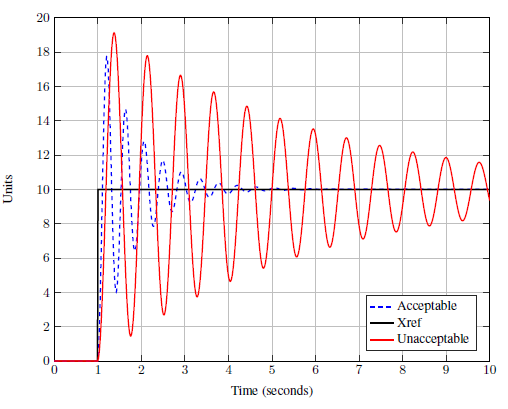
\includegraphics[width=.6\textwidth]{Figs/settime.PNG}
    \caption{Settling Time}
    \label{fig:settime}
\end{figure}
\paragraph{} In \citep{kapinski2016st} J.Kapinski et al provided an STL formalization for above property. Since all of them are defined in response to an asynchronous step input they extended the STL language to provide the operator
\begin{center}
$step(x,a) \triangleq x(t+\epsilon) - x(t) > a$
\end{center}
where $a$ is the step amplitude and $\epsilon$ corresponds to the smallest time variation following $t$. 
In the case the formula has to be verified by a discrete time monitors $\epsilon$ is equal to the sample time.
\par In STL, timed formulas can be nested such as, for example,
\begin{center}
$\lozenge_{[0, T]}(\textbf{q} \wedge \Box_{[a,b]} \textbf{p})$
\end{center}
The proposition $\textbf{p}$ is nested one level deeper than proposition $\textbf{q}$. The meaning is that there has to be one time instant $t$ in $[0,T]$ (the outer Eventually condition) such that $\textbf{q}$ is satisfied in $t$ and for all the system evolutions starting from time $t$, the condition $\textbf{p}$ is verified at some time between $t + a$ and $t + b$. In a runtime monitor implementation, the evaluation of the global condition with $\textbf{p}$ depends not only on the time range of its temporal operator, but also on the time $t$ in which $\textbf{q}$ is satisfied. If $t_q$ is the time at which $\textbf{q}$ is satisfied, the time range in which $\textbf{p}$ is evaluated becomes $[a + t_q , b + t_q]$. The nested time interval $[a , b]$ is therefore not an absolute time, but is relative to the time instant identified by the outer clause.
\paragraph{}The STL expression of the performance requirements comes in a more readable shape if formulas aim to prove the presence of the property instead of their absence:  
\begin{center}
\begin{tabular}{ll}
$RiseTime(ref,x,a,t_1,x_1)$ & $\lozenge_{[0, T]}(step(ref, a) \wedge \Box_{[0,t_1]}(x < x_1)) $\\
$FallTime(ref,x,a,t_1,x_1)$ & $\lozenge_{[0, T]}(step(ref, a) \wedge \Box_{[0,t_1]}(x > x_1)) $\\
$Overshoot(ref,x,a,x_2)$ & $\lozenge_{[0, T]}(step(ref, a) \wedge \lozenge (x - ref > x_2)) $\\
$Undershoot(ref,x,a,x_2)$ & $\lozenge_{[0, T]}(step(ref, a) \wedge \lozenge (ref - x > x_2)) $\\
$SettlingTime(ref,x,a,t_2,x_3)$ & $\lozenge_{[0, T]}(step(ref, a) \wedge \lozenge_{[t_2,T]} (|x - ref| > x_3)) $\\
\end{tabular}
\end{center}
where $T$ is the simulation time, $ref$ is the command to the system and $x$ is its output. In \textbf{REF} each pattern is coupled with a natural language representation, doing so we create the connection from natural to formal language, avoiding, at least for this class of requirements ,ambiguities and errors. 

\section{The Contract Paradigm}

The contract-based paradigm, founded on the use of contracts as formal requirements, allows distributed designers to develop different aspects and components of the overall system in a concurrent but controlled way. In a component-based model, a component is a hierarchical entity that represents a unit of design and components are interconnected and communicate through ports carrying discrete or event values. Implementations and requirements can be attached to components, where requirements are expressed as \textit{contracts} \citep{benveniste2007multiple,benvenuti2008contract}. A contract is an assertion on the behaviors of a component (the promise) subject to certain assumptions. An assertion represents a set of runs of the component and a run can be seen informally as a sequence of values of the component’s variables and ports. Therefore a contract $C$ is the pair of assertions
\begin{center}
$C = (A,G)$
\end{center} 
where $A$ corresponds to the assumption, and $G$ to the promise. The component’s contract $(A,G)$ corresponds to the requirement $A \rightarrow G$ or equivalently $G \cup \neg A$ on the implementation of the component. A component’s implementation $M$ satisfies the requirement if $M \subseteq G \cup \neg A$, in which case the implementation is said to satisfies the contract. 
\paragraph{} With reference to both requirements of \ref{en:ptreq}, the assumption under which system performances have to be validated is specified in the subsentence \textit{"...with a system inertia less than or equal to $S_{In}$"}. In fact it represents the environmental condition under which the system has to guarantee a specific behavior. By coupling the definition of domain patterns with the contract formalization those requirement can be restructured as follows
\begin{table}[h]
\centering
\begin{tabular}{|l|rll|}
  \hline \rule{0pt}{3ex}
Req. ID & \multicolumn{2}{c}{Formalization $C=(A,G)$} & \\
  \hline \rule{0pt}{3ex}
$R.01$ & $(inertia \leq S_{In} , $&$\neg RiseTime(ref,x,a,t_1,x_1) $&$\wedge$ \\ 
  & & $\neg Overshoot(ref,x,a,x_2) $&$\wedge$ \\
  & & $\neg SettlingTime(ref,x,a,t_2,x_3)$&) \\
  \hline \rule{0pt}{3ex}
$R.02$ & $(inertia \leq S_{In} , $&$\neg FallTime(ref,x,a,t_1,x_1) $&$\wedge$ \\ 
  & & $\neg Undershoot(ref,x,a,x_2) $&$\wedge$ \\
  & & $\neg SettlingTime(ref,x,a,t_2,x_3)$&) \\
  \hline 
\end{tabular}
\caption{Formalized Performance Requirements}
\end{table}

In complex models with multiple entities the interactions can be regulated by contracts of single components. Moreover, the system specification and validation can be conduced by combination of all components' assumptions and guarantees. Benveniste et al in \citep{benveniste2007multiple} provide different modalities of combining requirements expressed as contracts.

\paragraph{} It is common that each requirement reflect the interpretation of the customer needs related to a single aspect of the design and under some implicit or explicit hypothesis, that represents the precondition under which the behavior described in the requirement should be guaranteed. These \textit{preconditions} do not represent the system’s assumptions since they are not absolute constraints that the environment must satisfy. Instead, they model the enabling conditions under which the proposed behavior must be exposed by the system. As example, such preconditions are identified in performance requirement by the verification of a step input, since it acts as trigger for the evaluation of the effective promise related to the property. In \citep{mangeruca2013formalization} Mangeruca et al deeply analyze this difference, providing also a richer definition of the classical contract paradigm as the triple
\begin{center}
$C = [A, (P, Q)]$
\end{center}
where $A$ is the assumption, $P$ is the precondition and $Q$ is the guarantee. The newer semantics of the contract is then represented by the logical formula $A \rightarrow (P \rightarrow Q)$. For an in-depth exploration of such extended contracts please refer the reading.
\chapter{The Framework}

\section{From Requirements to Monitors}

The components structure of the developed framework is shown in Fig. \ref{fig:tool}.
\begin{figure}[!h]
	\centering 
     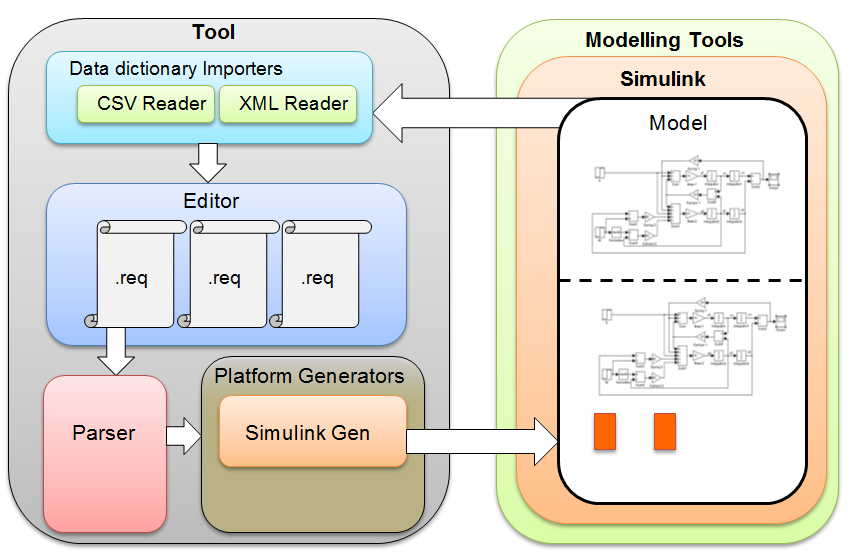
\includegraphics[width=.9\textwidth]{Figs/tool.PNG} 
     \caption{Requirement Framework} 
     \label{fig:tool} 
\end{figure}
\paragraph{Model to Tool} The tool cooperates with a modeling environment through two actions. The first consists of using a model reader to import the list of all model's signals and parameters into a data dictionary. This allows to write requirement referring entities directly with the same names as they are specified in the model. In addition to names, the import phase concur to gather information about data types, boundary values and measuring units.
\paragraph{Tool to Model} The second actions consists of populating the model with monitors generated out of the requirements. Such action is strictly dependent on the platform on which the model is defined. For this reason the tool has been designed to be as flexible as possible, by providing a set of \textit{{Platform Generators}} modules, each one for a specific target platform. In general, in order to ease its task, a platform generator could be supported with some platform libraries enclosing either operators or atomic instructions. In the case of Simulink the produced result is a script which, once executed, adds new requirements blocks to the provided model.
\paragraph{The Editor} In order to write requirements the tool offers a smart editor. It provides the most common user relieving features, such as the context-aware syntax completion ad coloring. Requirements are written according to a specific loose syntax, which is basically equivalent to an ordered sequences of natural language keywords. Even in this case, due to the large variability of possible syntaxes, the tool shows flexibility and provide support for syntax updates with very low effort.
\paragraph{The Parser} The syntax accepted by the editor is not as formal as a the one of a programming language, this complicates not a little the translation of a requirement as it is written. Therefore, before being delivered to a platform generator, the content of a requirement document is transformed into a syntax tree by means of a \textit{Mid Level Parser}. This action, although adds a further step to the synthesis process, ease the task of the platform generator since restructures its input in order to be programmatically analyzable.
\paragraph{} Following sections describe in depth all the components. As first version the tool support interactions only with Simulink, which is one of the most used modeling tools. However, for the sake of completeness, during explanation particular attention will be pose to emphasize all techniques adopted, during the development, to enforce extensibility of the tool. For this reason, also a brief survey of common Design Patterns will be conduced in \ref{sec:designpattern}.

\subsection{Syntax Definition}
\label{ssec:editorsyn}

The syntax of a requirement document has been developed in order to define requirements as contracts, the guarantee will be referred as an assertion, while the concept of precondition has not been explicitly used.
\par The grammar of the syntax is proposed as a list of recursive rules, each mandatory rule is enclosed within angular parentheses, while an optional one is enclosed within square parentheses. At the end of the recursion, rules are primitive, in the sense that they could be expressed through primitive data types (String, Integer, \dots). 
\noindent
\\
The entire syntax is defined as follow
\begin{lstlisting}[language=C]
Requirement Document = <Requirement List>
Requirement List = <Requirement>[Requirement List]
Requirement = <Header><Assumptions Section><Assertions Section>
Header = <ID><Title>
ID = 'R'<Requirement Number>
Requirement Number = <unsigned int>['.'Requirement Number]
Title = <string>
Assumption Section = <"ASSUMPTION"><Assumption List>
Assumption List = <Assumption>["AND" Assumption List]
Assumption = <Comparison statement> | <Signal Generator> | <Reference>
Comparison Statement = <Signal ID><Intermission><Comparison-op><SPV>
SPV = <Signal ID> | <Parameter ID> | <Value>
PV = <Parameter ID> | <Value>
Signal ID = FROM_DATA_DICT
Parameter ID = FROM_DATA_DICT
Value = <double>
Intermission = [Free-text]<"is" | "not">[Free-text]
Free-text = <string>
Comparison-op = <L_EQ> | <G_EQ> | <EQ>
L_EQ = <"less than">["or" EQ]
G_EQ = <"greater than">["or" EQ]
EQ = <"equal to">
Signal Generator = <Signal ID><"is"><Generator Type>
Generator Type = <Step> | <Ramp>
Step = <Step Type><"with amplitude"><PV><"beginning in"><PV>
Step Type = <"step"> | <"downstep">
Ramp = <"ramp with amplitude"><PV><",duration"><PV><"beginning in"><PV>
Reference = <Signal ID><"is reference">
Assertion Section = "ASSERTION"<Assertion List>
Assertion List = <Assertion>["AND" Assertion List]
Assertion = <Control Assertion>
Control Assertion = <Overshoot> | <Undershoot> | <Rise_Fall Time> |       <Settling Time>
Overshoot = <Signal ID><"overshoot shall be less than"><PV>
Undershoot = <Signal ID><"undershoot shall be greater than"><PV>
Rise_Fall Time = <Signal ID><"shall"><Rise_Fall><"from"><PV><"in less than"><PV>
Rise_Fall = <"rise"> | <"fall">
Settling Time = <Signal ID><"time to settle to"><PV><"shall be less        than"><PV>
\end{lstlisting}

\section{Support from Modeling Environment}

The cooperation of the requirements tool with a modeling environment could be easier if from the latter's side are provided some utilities. A good practice when writing requirements is to fill a data dictionary with system's components names and always refer them with that. To enforce the use of a data dictionary a modeling environment may offer the capability to partially generate it by exporting all entities in the model. From the other side, the process of auto-generate monitors for a targeted modeling environment can be lightened if the requirement tool could make use of built-in libraries. The libraries used to provide support for monitors generation have been already described in \citep{bals2017}. Since this thesis is meant as continuation of that work such libraries are reanalyzed, possibly providing further details, also in this context. Next sections explore in a more detailed way these utilities, providing also examples in the case of Simulink.

\subsection{Signal Exporter}

A Simulink model can be view as a collection of connected blocks, where each connecting line represents a signal. In complex models the number of signals is in the order of thousands. The environment allow to name every signal but, for the sake of practicality, does not force users to do so. Although naming, at least the more significant, signals indisputably represents a good modeling practice, rarely professional models comply with such rule. The common situation is that in real models names are provided only for blocks and subsystems' ports, which are not allowed to be unnamed.
\paragraph{} In order to be effective, a good Simulink signals exporter cannot avoid to consider the above aspect. In other words, it cannot rely on the fact that all meaningful signals' lines are named, and, somehow, has to overcome this problem. As possible solution, the signals exporter can, in first instance, collect all the lines' names and then continue with all the subsystems' output ports' names. Such approach allows to pick up a broad number of signals' names, however, it does not prevent from possible inconsistencies. As example, it does not produce results for models not defining subsystem blocks and for which no names are associated to lines. Further, since it prioritize lines rather than ports, for models in which a line and a port have the same name, which is perfectly legal in Simulink, the exporter will consider just one name for both. These limitation, however, represents borderline situations which are also deprecated by modeling practices.
\paragraph{} A signals exporter can be implemented with the following Matlab function, it requires as input the model and the file to fill with the signals' names. 
\begin{lstlisting}[language=MATLAB]
function signalExport(sys, fname)
    ssys = find_system(sys, 'BlockType', 'SubSystem');
    ssys = {sys,ssys{1:end}}';
    lines = find_system(ssys,'FindAll','on','type', 'line');
    signals = containers.Map;
    for i=1:length(lines)
        conn = get_param(lines(i), 'Connected');
        name = get_param(lines(i), 'Name');
        if (size(name, 2) > 0 && strcmp(conn, 'on'))
            signals(name) = 1;
        end
    end
    ports = find_system(ssys, 'BlockType', 'Step');
    ports = [ports ; find_system(ssys, 'BlockType', 'Ramp')];
    ssys = ssys(2:end);
    ports = [ports ; find_system(ssys, 'BlockType', 'Outport')];
    onames = get_param(ports ,'Name');
    t = isKey(signals, onames);
    allkeys = [keys(signals) onames(t==0)'];
    signals = containers.Map(allkeys, ones(length(allkeys),1));
    file = fopen(fname,'a+');
    k = keys(signals);
    for i=1:length(k)
        fprintf(file, 'signal,%s,,,,,\n', strjoin(k(i)));
    end
    fclose(file);
end
\end{lstlisting}
In addition to line and subsystems' outputs, it further refines the collection including also names of particular signals generation block, i.e. \textit{Step} and \textit{Ramp}. The choice of these two block is motivated by the fact that inside the editor's syntax (\ref{ssec:editorsyn}) there is an explicit reference to these kind of signal. The exporter can be extended as will simply adding clauses for new block types, as interesting new candidates, signal generators available in Simulink are the \textit{Pulse Generator} and the \textit{Sinusoidal Wave}.
\par It's possible to notice that the functions write the file according to a CSV format. This choice is dependent on the way the requirements tool expects to import data dictionaries, and will be clarified in section \ref{sec:datadictimp}.

\subsection{STL operators library}
\label{ssec:STLib}

In order to generate online monitors, the following restrictions has been introduced to the STL language.
\begin{enumerate}
\item The maximum level of nesting for temporal operators is two.
\item If there is a nested temporal operator, the condition on which the outer operator is evaluated must be a conjunction and at least one of the terms of the conjunction must be a proposition (not a temporal operator).
\item If $T_b$ is the maximum value for all the endpoints of the intervals defined in the inner (nested) temporal operators, then the terms of the conjunction that are not temporal operators can only be true at time instants that are separated by a time interval always greater than $T_b$. 
\end{enumerate}
\noindent
\\
The STL operators library implements a Simulink version of the \textit{And} plus the most common STL operators (Fig.\ref{fig:stlib}). 
\begin{figure}[!h]
	\centering 
     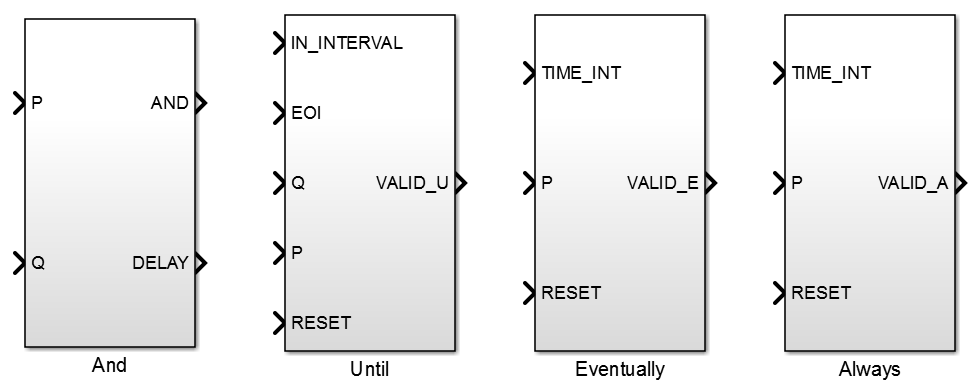
\includegraphics[width=.8\textwidth]{Figs/stlib.PNG} 
     \caption{STL Simulink} 
     \label{fig:stlib} 
\end{figure}
\noindent
\\
The \textit{And} block is needed to implement nested temporal operators, in particular, it represents the conjunction among outer and inner propositions. Despite the name, it is quite different from the classical logical And since it does not returns \textbf{true} if $P$ and $Q$ are \textbf{true} at the same time, but rather if $Q$ becomes \textbf{true} at some the time $t$ after $P$ became \textbf{true}. In order to verify $Q$ it returns, through the $DELAY$ port, the time in which $P$ was verified, such time is needed to correctly compute the interval of the $Q$'s temporal operator.  

\paragraph{} All the operators blocks keep their output constant after a the property is detected. However,  to facilitate their use in simulations concatenating several test cases, a reset input is also provided. Fig. \ref{fig:testSTLALEV} shows two test cases for \textit{Always} and \textit{Eventually}, one causing them return true and one false. 
\begin{figure}[h]
    \centering
    \begin{subfigure}[b]{0.48\textwidth}
        	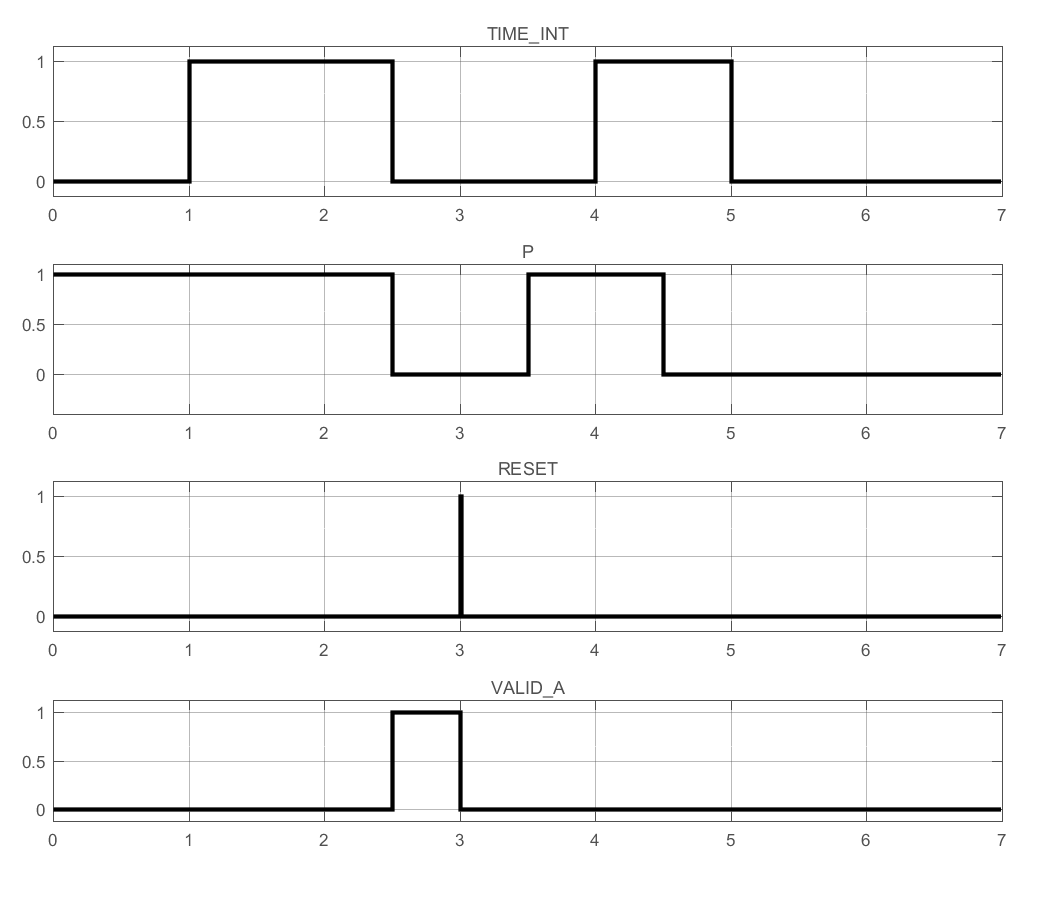
\includegraphics[width=\textwidth,height=188px]{Figs/testalw.eps}
        	\caption{Always}
            \label{fig:testalw}
    \end{subfigure}
        \begin{subfigure}[b]{.48\textwidth}
        	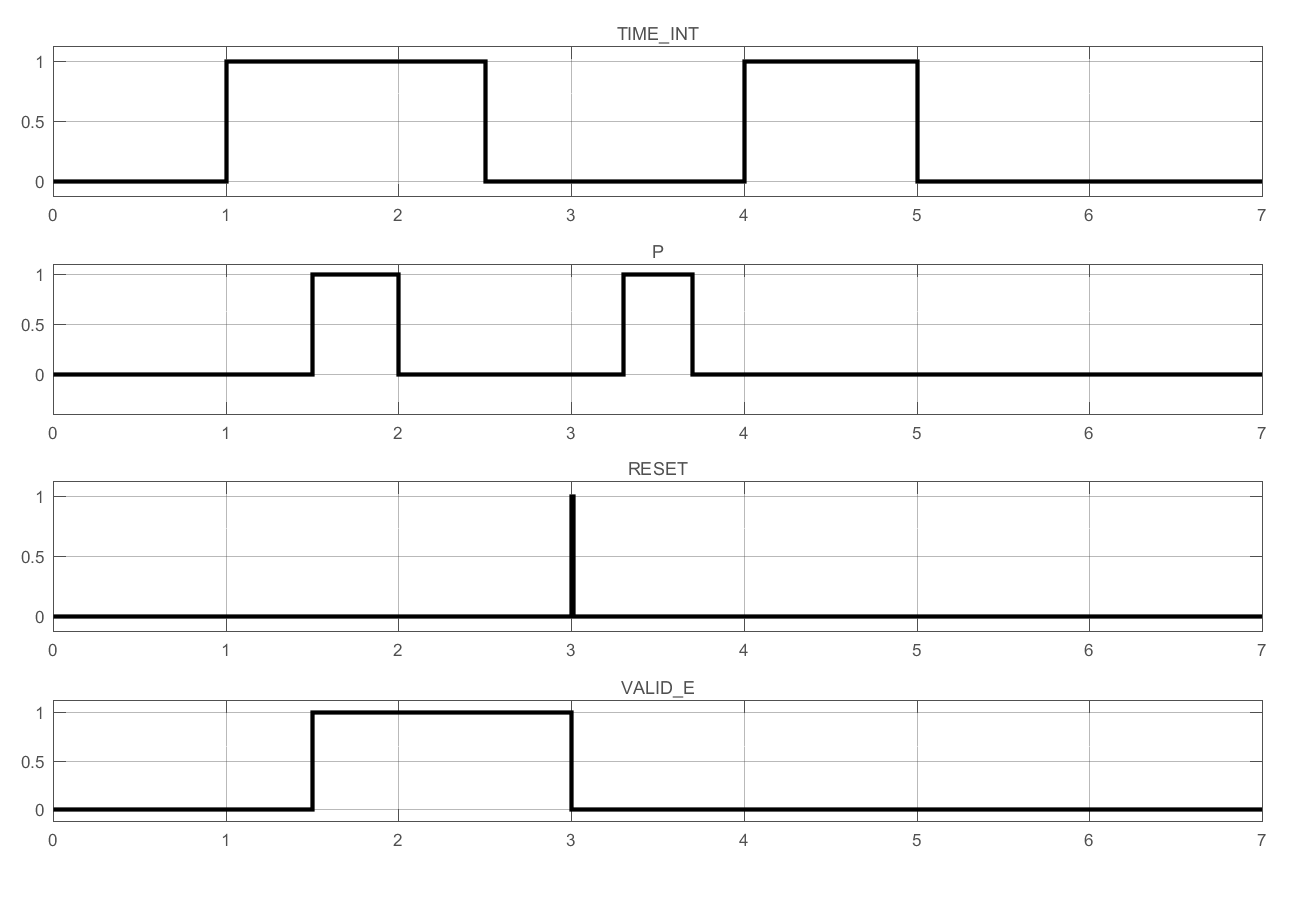
\includegraphics[width=\textwidth,height=188px]{Figs/testev.eps}
        	\caption{Eventually}
            \label{fig:testev}
        \end{subfigure}
    \caption{Test of STL Always-Eventually}
    \label{fig:testSTLALEV}
\end{figure}
\noindent
\\
In particular, it is possible to notice that the two operators have different behaviors due to their dynamics. The Always produces positive outputs only at the end of the time interval relative to the current test case  (Fig.\ref{fig:testalw}). Conversely, the Eventually operator returns positive feedback immediately after the occurrence of a positive input  (Fig.\ref{fig:testev}).
\par Compared to its brothers, the timed \textit{Until} operator has a more complex dynamics, in fact, in presence of multiple test case during the same simulation, it is not possible to determine a priori the instant in which it reacts to each input sequence. Fig. \ref{fig:testunt} present a possible multiple cases simulation for the timed Until.
\begin{figure}[!h]
	\centering
    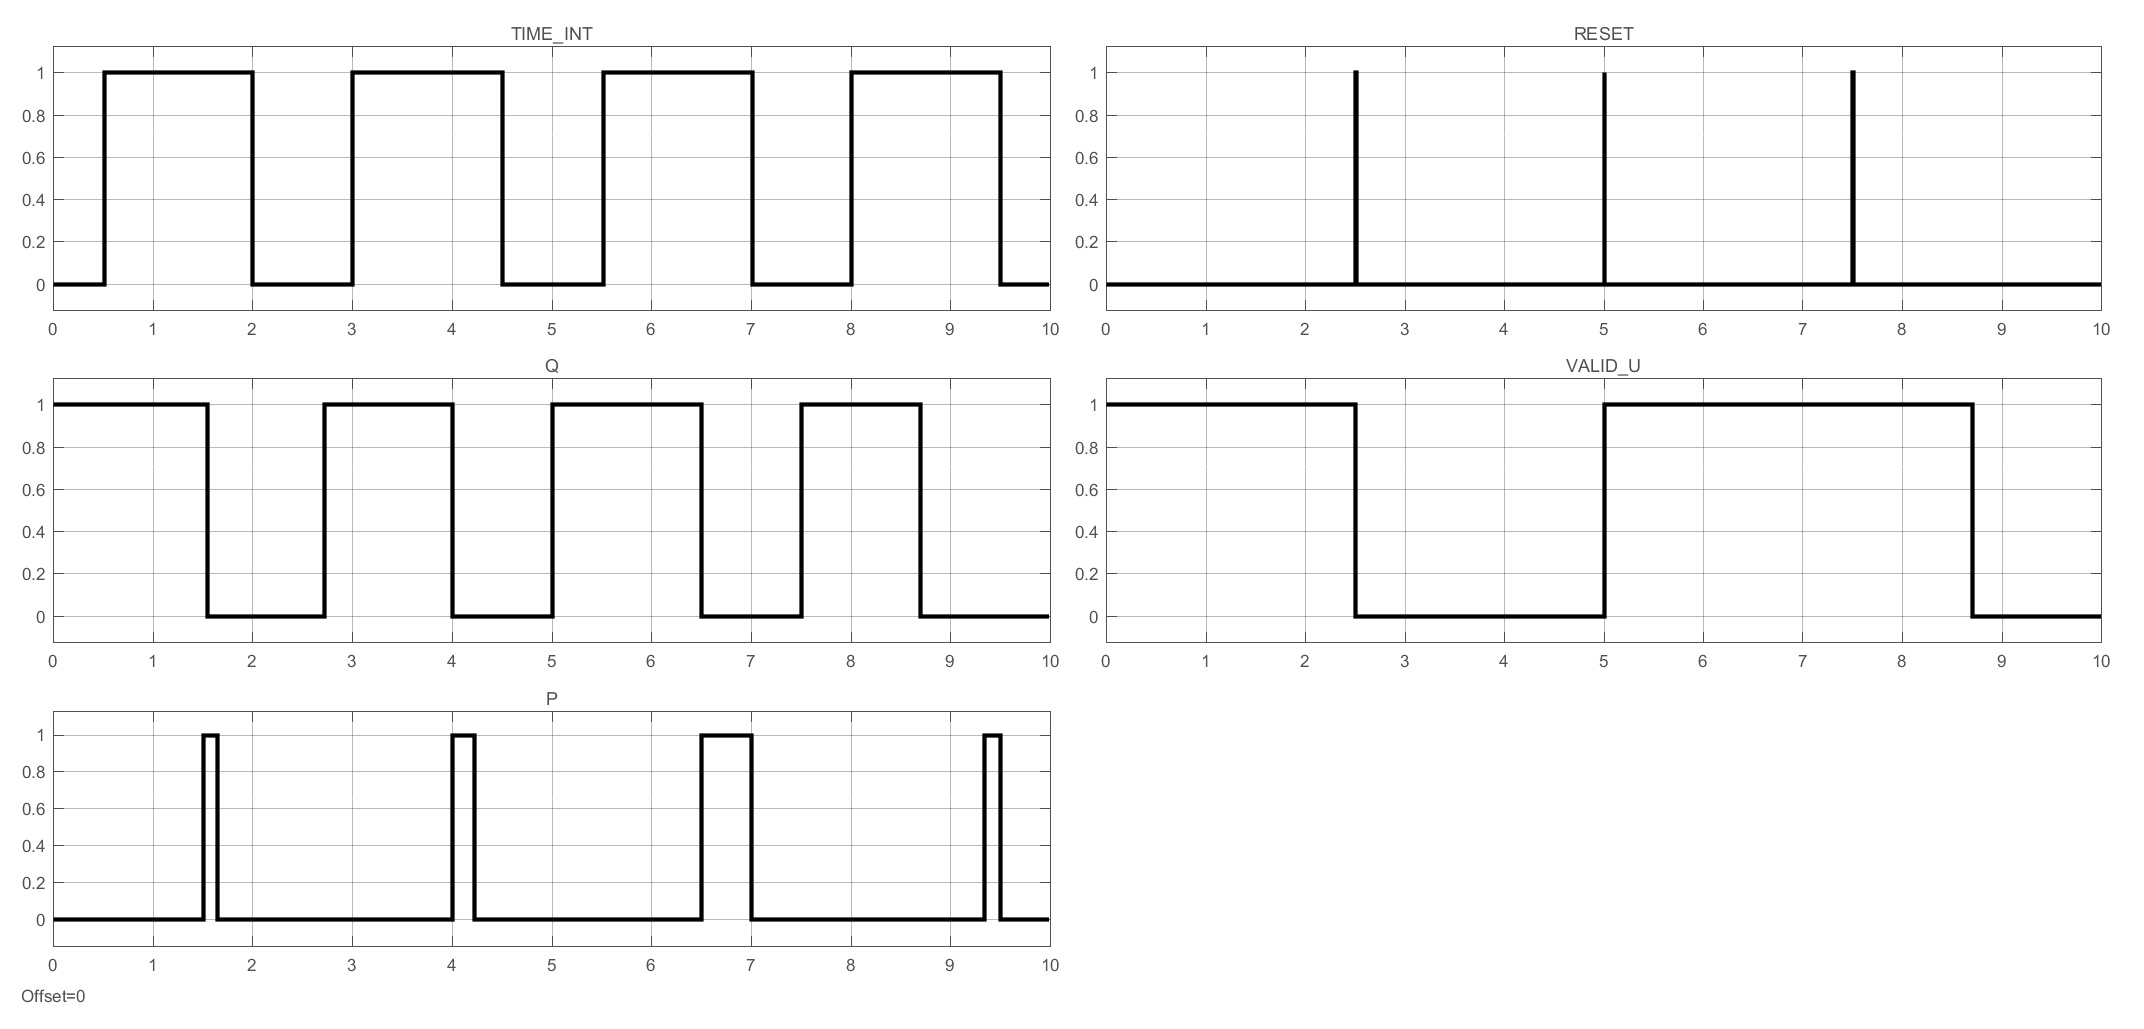
\includegraphics[width=\textwidth]{Figs/testunt.eps}
    \caption{Until Simulation}
    \label{fig:testunt}
\end{figure}
\noindent
\\
The operator returns true if within a time interval the proposition $P$ is true at least once and, for all the time before this happen, the proposition $Q$ is true. The simulation provide four different time intervals. For the first, the operator always returns true since $Q$ is always true until $P$ becomes true. For the second interval, it immediately returns false since, after the reset, the proposition $Q$ is false. After the second pulse of signal reset the operator returns again true, indeed this scenario is perfectly analogous to the first one. During the last time interval, there is yet another behavior. The operator is not immediately returning false, $Q$ is true after the reset, but rather when $Q$ becomes false since $P$ has not yet became true. Note that another behavior, which has not been included for the purpose of not overload the graphics, is observable for the edge case in which $Q$ is always true within a reset and the end of a time interval, and $P$ is always false in the same time. In this case the operator reacts with a negative output only at the end of the time interval, since, till the end , it "waits" for $P$ becoming true.
\paragraph{} The Simulink implementation of the STL timed Until is depicted in Fig. \ref{fig:untimpl}. The other operators are implemented in a similar, and simpler, shape. The complete library is available at \citep{balsrepo}.
\begin{figure}[!h]
\centering
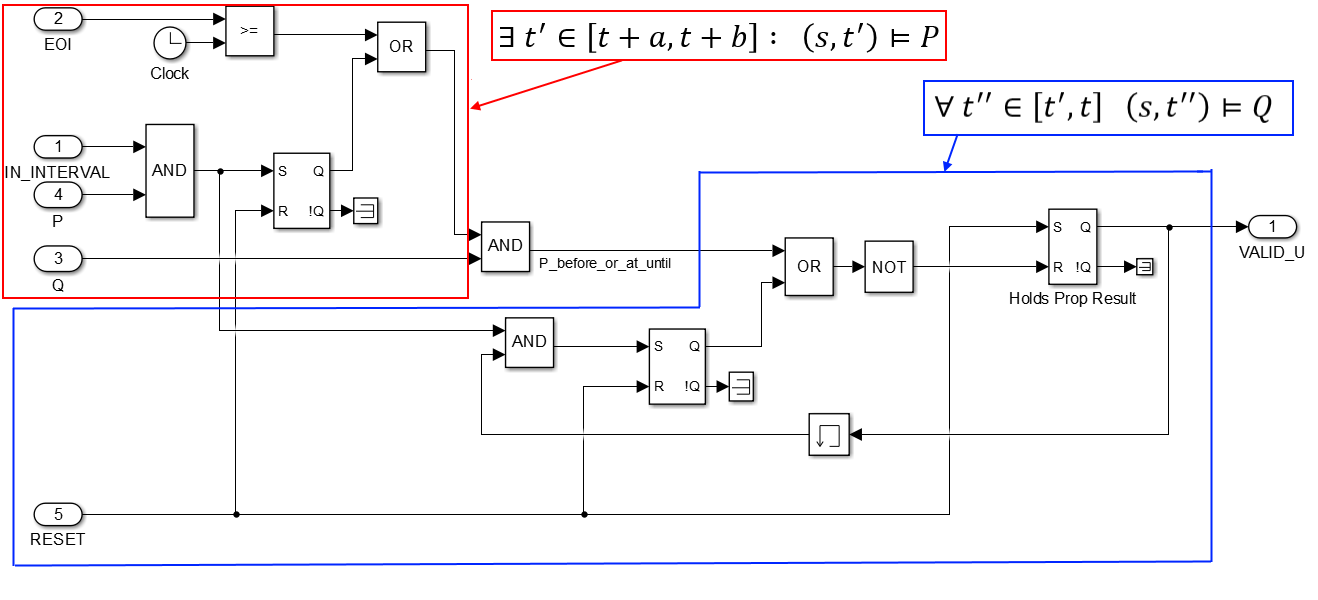
\includegraphics[width=\textwidth]{Figs/untimpl.png}
\caption{Timed Until Implementation}
\label{fig:untimpl}
\end{figure}

\subsection{System Performance Control Library}

Section \ref{ssec:dompatterns} provided an STL formalization of the most common control system performance requirements. In the same has been argued that such formalizations represent patterns, namely parameterizable properties having a fixed formal structure. Offering an implementation of those pattern is the main purpose of the \textit{System Performance Control Library} (SPCL), it provides several atomic blocks able to verify the violation of performance requirements.The library block-set is presented in Fig. \ref{fig:spctrlib}. 

\begin{figure}[h]
\centering
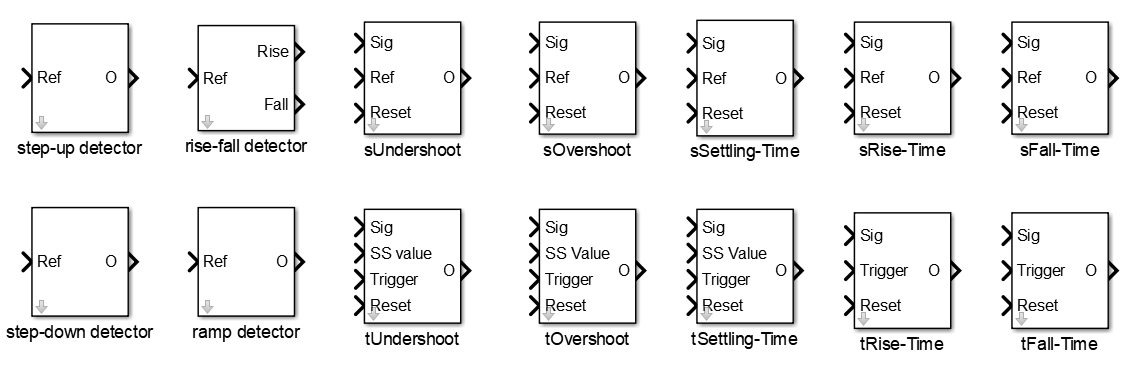
\includegraphics[width=\textwidth]{Figs/spclib.PNG}
\caption{System Performance Control Library}
\label{fig:spctrlib}
\end{figure}

The entire block-set has been developed to operate in a simulation environment that uses a fixed-step solver for \textit{ODE} integration. Possible future versions of the library will eliminate such limitation, allowing their use with a variable-step solver, by simply forcing the user to set a sample time for the block to discretize time and input signals.
\paragraph{} A first categorization of all blocks could be performed by dividing them in \textit{checkers} and \textit{detectors}. Checker blocks, as the name suggest, are those in charge of effectively assert the violation of the property. In order to do so, they need to cooperate with the detectors blocks, which are pulse emitters based on the behavior of their input signals. The cooperation between detectors and checkers can be \textit{implicit} or \textit{explicit}, and allows to split the latter into two more subcategories depending on the type. 
\par Blocks belonging to the first, whose name starts for "\textit{s}", internally perform the classification of the input type by means of a step (up or down) detector. Therefore, those blocks direct implement the formulas of section \ref{ssec:dompatterns}. Ideally this subcategory is enough to verify performance requirements, since these properties are defined under the hypothesis of step as reference input. The reason why the library includes more general versions of this blocks, based on an explicit cooperation with an input detector, comes from the practical user experience. Indeed, many times, along multiple experiments, users may adopt reference signals sharing common features with steps, but having some substantial differences which makes them undetectable as steps. Two common examples are steps followed by a rate limiter (Fig. \ref{fig:ratelim}) and pulse generators (Fig. \ref{fig:pulsegen}). The first is typically used to avoid sharp changes on input and basically transforms a step into a ramp, while the second is used to provide multiple inputs since it can be view as a sequence of up and down steps.  
\begin{figure}[h]
\centering
\begin{subfigure}{\textwidth}
\begin{subfigure}{.48\textwidth}
\centering
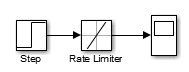
\includegraphics[width=.7\textwidth]{Figs/ratelim2.PNG}
\end{subfigure}
\begin{subfigure}{.48\textwidth}
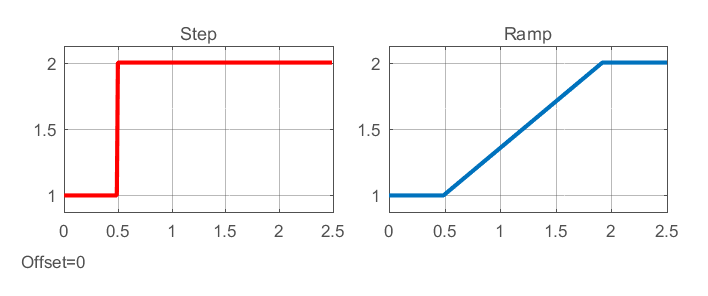
\includegraphics[width=\textwidth]{Figs/ratelimsim.eps}
\end{subfigure}
\caption{Rate Limiter}
\label{fig:ratelim}
\end{subfigure}
\begin{subfigure}{\textwidth}
\begin{subfigure}{.48\textwidth}
\centering
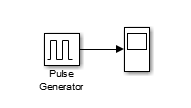
\includegraphics[width=.7\textwidth]{Figs/pulse.PNG}
\end{subfigure}
\begin{subfigure}{.48\textwidth}
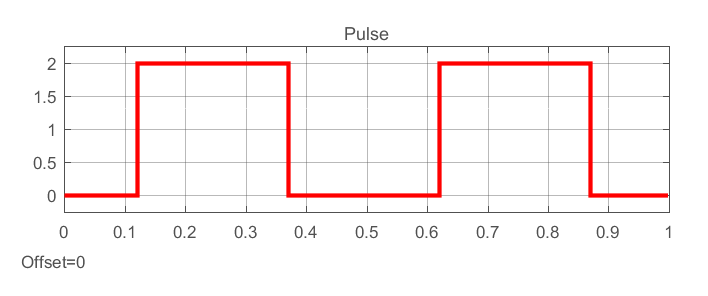
\includegraphics[width=\textwidth]{Figs/pulsesim.eps}
\end{subfigure}
\caption{Pulse Generator}
\label{fig:pulsegen}
\end{subfigure}
\caption{Input References}
\end{figure}
\noindent
\\
In order to support those kind of inputs, without forcing the user to modify existing model to comply with the library, the blocks  family starting with "\textit{t}" label can be used. Unlike the implicit blocks, in addition to the \textit{Trigger} produced by a detector some of them may need more information that normally can be inferred by the reference signal, like, for instance, the steady-state value.

\paragraph{Signal Detectors} As previously said, detectors blocks emit pulses every time the input signal shows an expected behavior. The parameter to evaluate the conditions are set from the user by means of the blocks' masks. In what follows will be focused just the step-up and the ramp detectors, step-down and rise-fall detectors are not considered since the first works reciprocally to the step-up while the second is just a parallel composition of a step-up and a step-down. 
\begin{figure}[h]
\centering
\begin{subfigure}[b]{.48\textwidth}
\centering
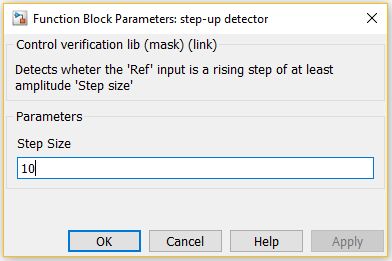
\includegraphics[width=\textwidth]{Figs/stepmask.PNG}
\caption{step-up detector's Mask}
\end{subfigure}
\begin{subfigure}[b]{.48\textwidth}
\centering
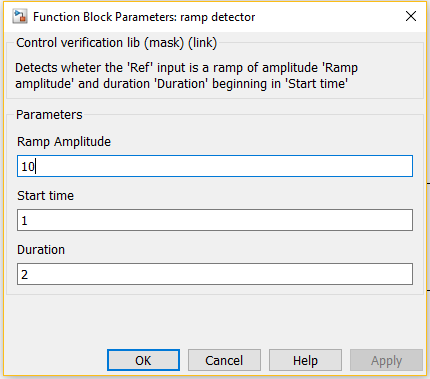
\includegraphics[width=\textwidth]{Figs/rampmask.PNG}
\caption{ramp detector's Mask}
\end{subfigure}
\caption{Detector's masks}
\label{fig:detmasks}
\end{figure}
From the blocks' masks (Fig.\ref{fig:detmasks}) is possible to note that step-up detector, unlike ramp-detector which requires start and duration time, has not parameter which are functions of time, this allow to use it multiple times in the same simulation. A possible time behavior for both detectors is shown in Fig. \ref{fig:detbehavior}, in the case of the step, due to the detectors definition, does not make difference if the input signal is a single step or a step train. Indeed, the detector implementation expects that it reacts every time there is a difference of at least \textit{Step size} between two time-consecutive samples of the input signal.
\begin{figure}[h]
\centering
\begin{subfigure}[b]{.48\textwidth}
\centering
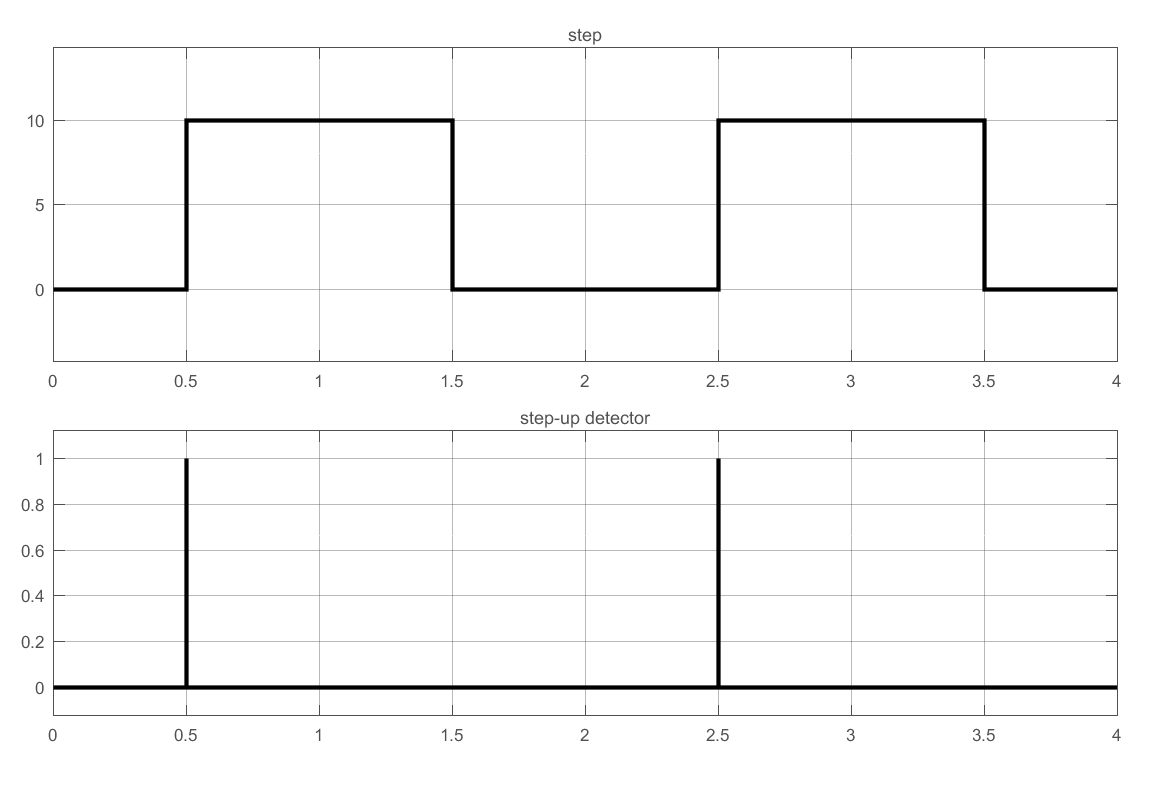
\includegraphics[width=\textwidth]{Figs/stepdetsim.eps}
\end{subfigure}
\begin{subfigure}[b]{.48\textwidth}
\centering
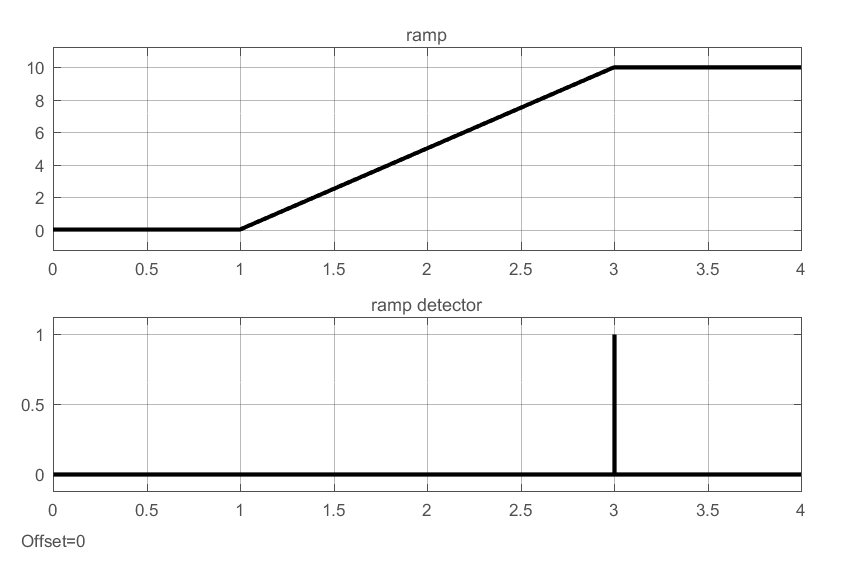
\includegraphics[width=\textwidth]{Figs/rampdetsim.eps}
\end{subfigure}
\caption{Detectors' time behavior}
\label{fig:detbehavior}
\end{figure}
The implementation of the ramp detector is more complex, it is based on the idea that the block must check if, for all $t$ in $[Start, Start+Duration]$, the input signal is a line with a slope equal to $\frac{Amplitude}{Duration}$. This definition can be formally written with the following STL

\begin{center}
$\Box_{[St, St+Dur]}\Bigg\{\dfrac{dx}{dt}==\dfrac{Ampl}{Dur} \Bigg\}$
\end{center}

Such formula can be easily implemented with the Always operator of the STLib (\ref{ssec:STLib}). Please note that in the real implementation (Fig.\ref{fig:rampdetimpl}) the equality of slopes is not checked through the equal operator, but rather ensuring that their difference is less than a very small quantity. This approach has been adopted to avoid possible numerical issues on determining the exact equality of two numbers.
\begin{figure}[ht]
\centering
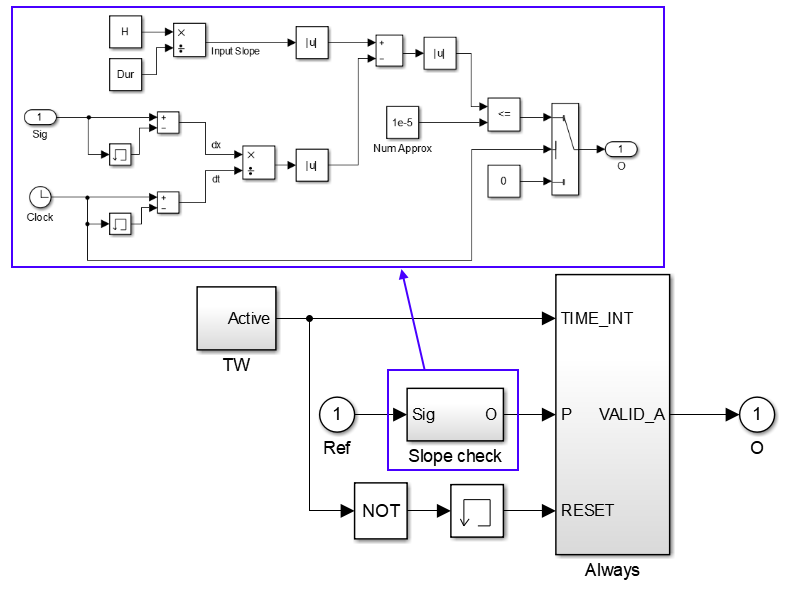
\includegraphics[width=\textwidth]{Figs/rampimpl.png}
\caption{Ramp Detector Implementation}
\label{fig:rampdetimpl}
\end{figure}
\paragraph{Property Checkers} For each performance requirements the library provides two different blocks depending on the type of cooperation with a signal detector. Time behavior and internal structure of blocks-couples relative to each property are very similar. Therefore, without losing generality only overshoot requirement will be analyzed as a case study.
\paragraph{} The property's parameters, provided through the blocks' mask, are slightly different in the case of implicit (Fig.\ref{fig:sovmask}) or explicit (Fig.\ref{fig:tovmask}) reference detection. Indeed, if the blocks has to internally perform the step-up detection it needs to know the step size. Conversely, if the block only receives a detection trigger such parameter is not needed anymore. However, in order for the latter working properly, the information needed to estimate the overshoot has to be provided through a further input port, which has been labeled as "\textit{SS Value}"(Fig.\ref{fig:spctrlib}). The common parameters of the two blocks are \textit{Tolerance}, which represents the maximum tolerated distance among \textit{Sig} and \textit{Ref} (or \textit{SS value}), and \textit{Interval Size}, which corresponds to the simulation time.
\begin{figure}[ht]
\centering
\begin{subfigure}[b]{.4\textwidth}
\centering
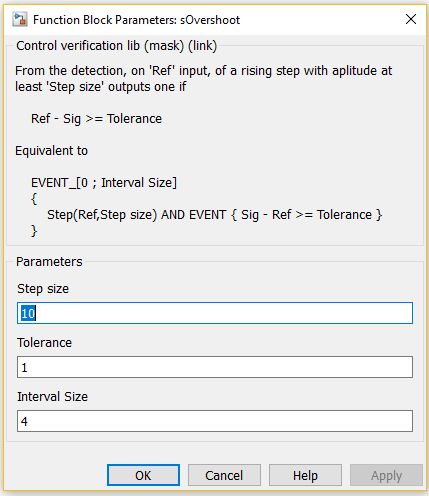
\includegraphics[width=\textwidth]{Figs/sovmask.PNG}
\caption{\textit{sOvershoot}}
\label{fig:sovmask}
\end{subfigure}
\begin{subfigure}[b]{.4\textwidth}
\centering
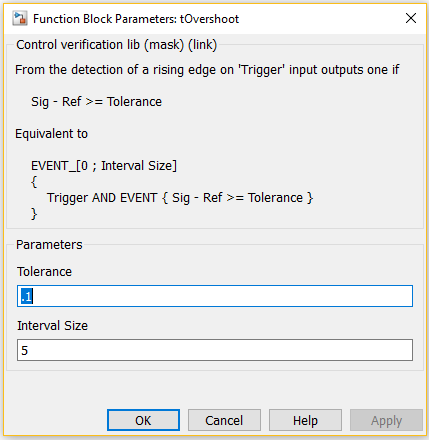
\includegraphics[width=\textwidth]{Figs/tovmask.PNG}
\caption{\textit{tOvershoot}}
\label{fig:tovmask}
\end{subfigure}
\caption{Overshoot Blocks' Masks}
\end{figure}
\paragraph{} Two possible simulations involving \textit{sOvershoot} and \textit{tOvershoot} are shown in Fig.\ref{fig:ovtresp}. For the first a step has been used as reference input, while for the second a ramp. Both blocks reacts immediately after the violation of the requirement.
\begin{figure}[!h]
\centering
\begin{subfigure}[b]{.45\textwidth}
\centering
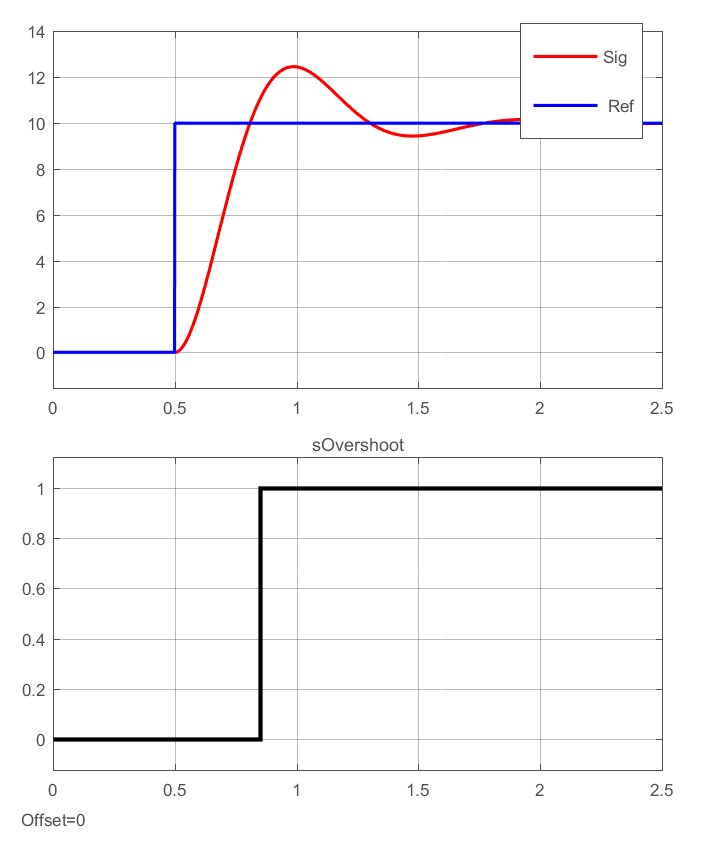
\includegraphics[width=\textwidth]{Figs/sovsim.eps}
\caption{\textit{sOvershoot}}
\end{subfigure}
\begin{subfigure}[b]{.45\textwidth}
\centering
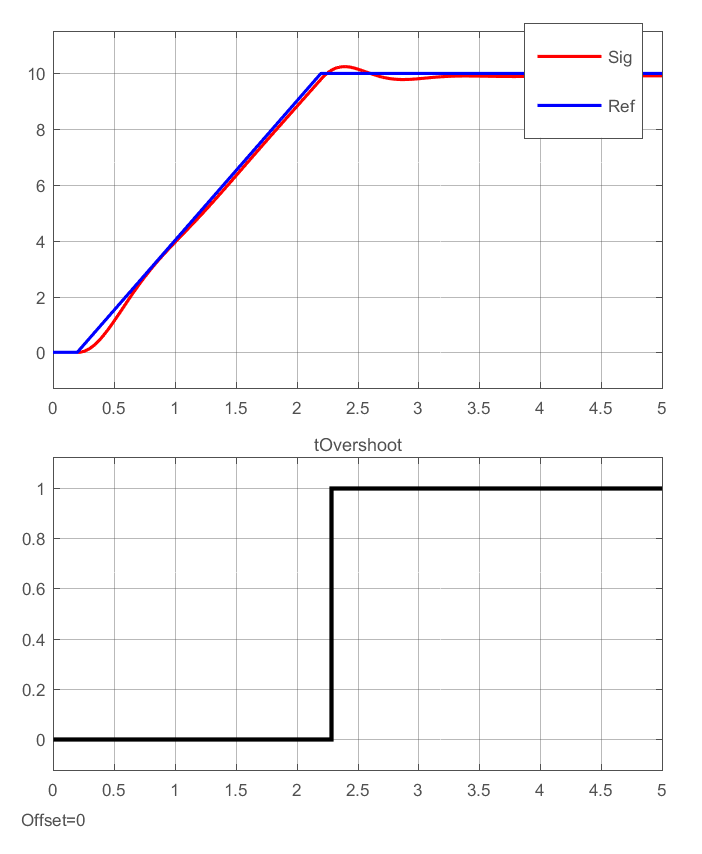
\includegraphics[width=\textwidth]{Figs/tovsim.eps}
\caption{\textit{tOvershoot}}
\end{subfigure}
\caption{Overshoots' Time response}
\label{fig:ovtresp}
\end{figure}
\noindent
\\
The blocks have a layered structure which recalls the level of nesting of the parent STL formula. Essentially, the Simulink implementation of the two blocks only differ for the signal used as first input of the \textit{And} operator inside the blocks' first layer (Fig.\ref{fig:ovimpl}). Such signal correspond to the proposition used at the left of the internal conjunction in nested STL temporal operators. Therefore, the STL formula, implemented in the \textit{tOvershoot} block, can be rewritten as 
\begin{center}
$\lozenge_{[0,T]}\big\{Trigger \wedge \lozenge \{ Sig - SSValue \geq Tolerance\} \big\}$
\end{center}

In order to avoid redundancy, the content of \textit{overshoot} subsystem of Fig.\ref{fig:ovimpl} has not been reported. Indeed, for both versions of the blocks, its structure is analogous to the first layer, i.e. an STL eventually with a less than or equal to proposition as input. 
\begin{figure}[!h]
\centering
\begin{subfigure}[b]{.48\textwidth}
\centering
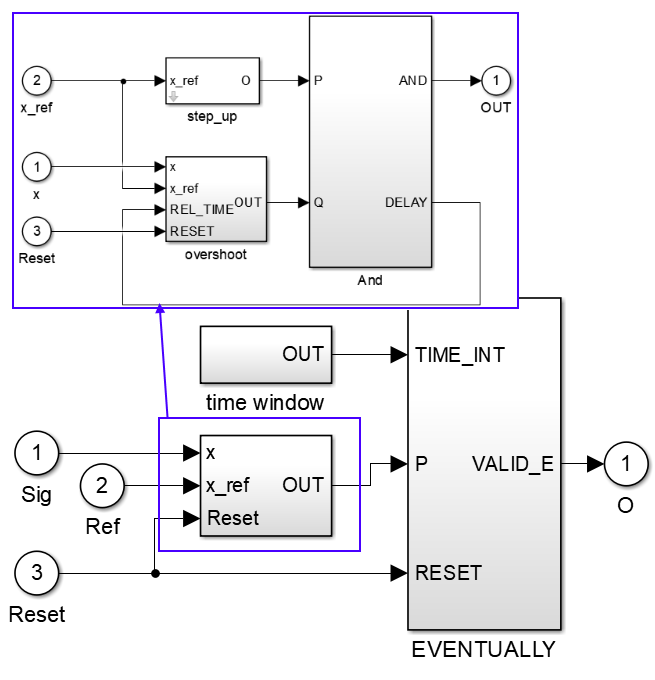
\includegraphics[width=\textwidth]{Figs/sovimpl.png}
\caption{\textit{sOvershoot}}
\end{subfigure}
\begin{subfigure}[b]{.48\textwidth}
\centering
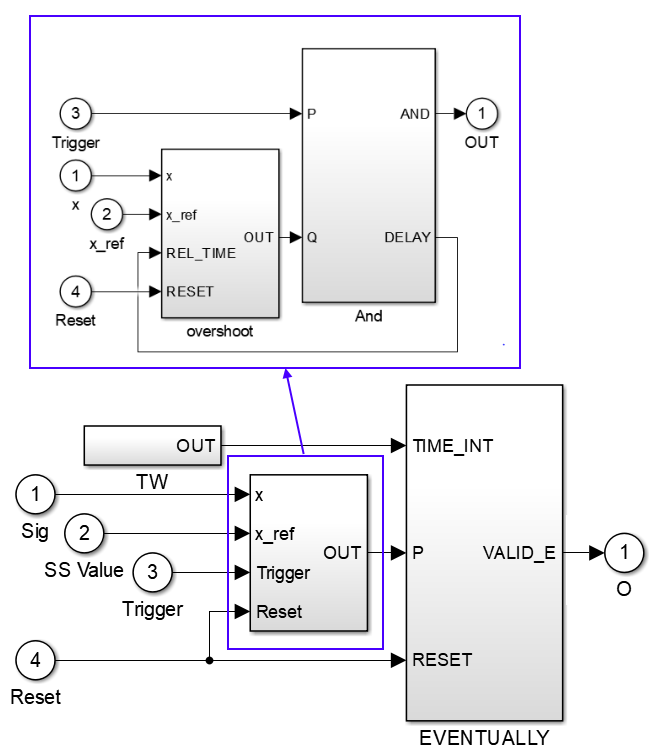
\includegraphics[width=\textwidth]{Figs/tovimpl.png}
\caption{\textit{tOvershoot}}
\end{subfigure}
\caption{Overshoots' Implementations}
\label{fig:ovimpl}
\end{figure}

All other property checkers follow the same philosophy of overshoot blocks. Although with them a good coverage of the performance requirements has been achieved, as future extension other properties may be included, making the \textit{SPCLibrary} a complete tool-chain for the analysis, during simulation, of several control systems models.

\section{Design Patterns}
\label{sec:designpattern}


In object-oriented software design a pattern describes a problem which occurs over and over in the environment, and then describes the core of the solution to that problem, in such a way that you can use this solution multiple times \citep{vlissides1995design}. Design patterns make it easier to reuse successful designs and software architectures, and helps avoiding design alternatives that compromise reusability.
\noindent
\\
Design patterns solve many problems that object-oriented designers face every day, like
\begin{description}
\item[Finding appropriate abjects] The hard part about object-oriented design is decomposing a system into objects. Design patterns help identifying abstractions and the objects that can capture them.
\item[Determining object granularity] Objects can vary tremendously in size and number.Design patterns address this issue as well. Many of them describe specific techniques of decomposing an object into smaller objects.
\item[Specifying object interfaces] Interfaces are fundamental in object-oriented software systems. There is no way to know anything about an object without going through its interface. Design patterns help defining interfaces by identifying their key elements and the kinds of data that get sent across an interface.
\end{description}
\noindent
\\
An exhaustive treatment of all known design patterns requires an huge effort, and leads to cover situation that are out of the scope of this work. Hence, herein only two of them, those really involved, will be taken into consideration. Being scalability and extensibility key factors of the proposed framework, particular care must be payed on the software architecture. The use of patterns belonging to \textit{creational} and \textit{behavioral} classes greatly helps to accomplish this objective. 

\subsection{Factory}

Creational patterns abstract the instantiation process. They help make a system independent of how its objects are created, composed and represented. A class creational pattern uses inheritance to vary the class that's instantiated, whereas an object creational pattern will delegate instantiation to another object. Creaional patterns become important as system evolve to depend more on object composition than class inheritance. As that happens,emphasis shifts away from hard-coding a fixed set of behavior toward defining a smaller set of fundamental behavior that can be composed into any number of more complex ones. Thus creating objects with particular behavior requires more than simply instantiating a class.
\paragraph{} The intent of the \textit{Factory Method} is defining an interface to create objects, but let subclasses decide which class to instantiate. The UML representation of the Factory pattern is shown in Fig.

\begin{figure}[h]
\centering
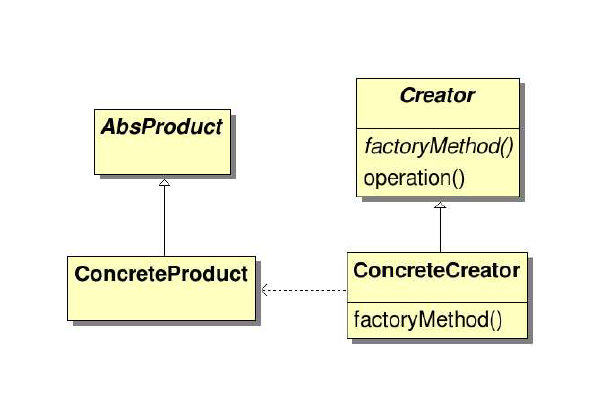
\includegraphics[width=.7\textwidth]{Figs/factory2.png}
\caption{Factory}
\label{fig:factory}
\end{figure}

\begin{description}
\item[Product] defines the interface of the objects the factory method creates
\item[Concrete Product] implements the Product’s interface
\item[Creator]declares the factory method
\item[Concrete Creator] overrides the factory method to return an instance of a
ConcreteProduct
\end{description}
\noindent
\\
Sometimes class Factories are implemented as \textit{Singleton}, which is another design pattern ensuring that in the system there is only one instance of the class. The client class request for the creation of new a new concrete product to the Factory and uses object through their interface. Typically the client provide to the Factory a products identifier, this is then used, for instance, inside a switch/case to determine the correct concrete product. However, managing all possible Concrete Products by hard-coding the logic to create them is not flexible. For this reason, more sophisticated techniques are usually adopted, they make use of the so called \textit{registry} and let Concrete Products register themselves into the factory. Follows an example of the Factory pattern, it make use of \textit{Reflections}, which is a Java mechanisms to discover information about the fields, methods and constructors of loaded classes, and to use reflected fields, methods, and constructors to operate on their underlying counterparts.

\begin{lstlisting}[language=Java]
interface Product {
	String getName();
}
class ProductOne implements Product {
	static {
		ProductFactory.instance().register("One", ProductOne.class);
	}
	public String getName() { return "instance of ProductOne"; }
}
class ProductTwo implements Product {
	static {
		ProductFactory.instance().register("Two", ProductTwo.class);
	}
	public String getName() { return "instance of ProductTwo"; }
}

class ProductFactory {
	// Singleton
	static private ProductFactory inst = new ProductFactory();
	static public ProductFactory instance() { return inst; }
	// The registry
	private HashMap registry = new HashMap();
	public void register(String productID, Class productClass) {
		registry.put(productID, productClass);
	}
	public Product create(String ID) {
		Class pClass = (Class)registry.get(ID);
		if (pClass == null) {
			System.err.println("Product " + ID + " not registered");
			return null;
		}
		try {
			Constructor pConstructor = pClass.getDeclaredConstructor(null);
			return (Product)pConstructor.newInstance(null);
		}
        ...
}
...
public static void main(String[] args)
{
	Class.forName("ProductOne");
	Class.forName("ProductTwo");
    ...
}
\end{lstlisting}
The Factory uses an associative set in order to couple Concrete Products with their identifier. Each Concrete Product register itself through the initial static block, however, in order to be sure of having all the registration done before start creating Concrete Product, the loader method "\textit{Class.forName(ClassName)}" has to be called.

\subsection{Visitor}


\section{Eclipse Editor}

\subsection{Data Dictionary Importer}
\label{sec:datadictimp}

\subsection{Context Aware Syntax Helper}

\subsection{Abstract Syntax Tree Generation}

\section{Model population}
\chapter{Conclusions}


The present thesis proposed a Model Based Design tool for system requirements validation and verification. It is possible to locate such framework in the first layer of a V-Model, where usually lie Top-Level (or User) requirements and Verification (or Validation) phases. Has been argued how these two stages can be coupled to enforce their correlation in therms of time and contents. The framework tries to automate such coupling, eliminating the effort for implementing the verification procedures. Moreover, it can be of help in finding the best way for the specification of the requirements itself. Such problem is known in the literature as Virtual Verification \citep{schamai2010virtual}, and can be view as an internal V-Model where the developed product is the requirements specification. Briefly, it expects the development of models which aims to verify textual requirements completeness and correctness.
\paragraph{} The framework comes with the main objective of providing a standard way to couple the usability of a textual representation with the effectiveness of a formal specification. Despite they requires strong technical skills, formal logics represent now-days one of the best way for product certification. The above gap has been reduced involving patterns, but, in order to consider it as a standard approach, a scalability analysis is still required.
\paragraph{} This work offers a proof of concept prototype. As such several features more on the side of classical requirements editors has been sacrificed in favor of a flexible coexistence with modeling environments. Even if in its first version the tool support cooperation only with Simulink, its internal structure allows in small time to experiment whether the approach could fit many others. Next section will discuss about several future works that can improve the overall tool potentiality.

\section{Future Work}

\paragraph{The tool} The requirements tool can be enriched of features exposed by several professionals requirements editors, such as DOORS \citep{DOORS}. Requirements can be hierarchically managed, this is particular useful when top-level requirements have a low-level representation which takes into account how, for instance, the property is mapped into the hardware. Another useful feature could be the capability of internally, or externally, link requirements. The internal links may represent some dependencies among requirements, while external link can be used to immediately point out some models or external file that provides a better explanation of the requirement. Further, a change tracking mechanism is another features that can help users to always have the complete history of the requirements, this is also useful in the process of virtual verification. Another potential service that the tool can provide is the read/write access to the data-dictionary. Since the syntax mostly provide sentences that has names as starting word, having the complete data-dictionary at disposal can help user to correct refer entities.

\paragraph{The Editor} In the current state the editor provides quite interesting capability of syntax coloring and completion. Particularly for the latter, the dynamic syntax loading into Tries is a capability that very easily allows to modify the suggestions. On the other hand the editor does not provide any features of syntax checking, this is surely a good starting point since it can enforce the work done by the syntax helper. Indeed, right now user does not have a real-time feedback for the syntax he is typing, but rather the helper stops providing suggestions if something is wrong in what typed. There are many possible way to implement a syntax checker module, the simplest one could be involving the use of a run-time regular expression marcher, however this at the end provides only a valid-invalid feedback and does not scale very well with the syntax's growth . A better solution could involve again the ANTLR parser, and the redefinition of its errors management strategies. This approach could add to the valid-invalid feedback also the reason of the result, that can be directly provided to the user in order to let him aware.  As a further, minor, improving many compact notation can be used in the syntax, for example numbers such as "0.000001" can be shortly represented as "1e-6". 

\paragraph{MBD features} Many improvements can come also for the MBD perspective. The contract-based formalization can be extended with the concept of precondition, this new section can replace or flank the assumption. Such refinement further enforce the unambiguousness of the requirement since better clarify roles inside it. More on the modeling side the interaction with environment can be improved by eliminating as much as possible the user intermissions. As an example the data-dictionary could be directly generated from a Simulink model without requiring the translation into supported file. Users simply provide as input of the importer a model file and it is converted into a data-dictionary, this features may involve the integration inside the tool of some archive decompressors and file managers. Another interesting feature could be having a real-time interaction with the modeling environment and the editor, which can mark satisfied and violated requirements.
\par The last, and perhaps the most important one, improvement is to extend compatibility with as much modeling environment as possible. Together with Simulink, modeling tools such as Scade \citep{Scade}, Scicos \citep{Scicos}, SysML \citep{sysml}, Modeler\citep{Modeler} and LabView \citep{Labview} find their application in several different domains, but the requirements specification is an omnipresent problem and the possibility to adopt the proposed framework in all these tool could be the key factor of this approach.

% ********************************** Back Matter *******************************
% Backmatter should be commented out, if you are using appendices after References
%\backmatter

% ********************************** Bibliography ******************************
\begin{spacing}{1}

% To use the conventional natbib style referencing
% Bibliography style previews: http://nodonn.tipido.net/bibstyle.php
% Reference styles: http://sites.stat.psu.edu/~surajit/present/bib.htm

\bibliographystyle{alpha}
%\bibliographystyle{unsrt} % Use for unsorted references  
%\bibliographystyle{plainnat} % use this to have URLs listed in References
\cleardoublepage
\bibliography{References/references} % Path to your References.bib file


% If you would like to use BibLaTeX for your references, pass `custombib' as
% an option in the document class. The location of 'reference.bib' should be
% specified in the preamble.tex file in the custombib section.
% Comment out the lines related to natbib above and uncomment the following line.

%\printbibliography[heading=bibintoc, title={References}]


\end{spacing}

% ********************************** Appendices ********************************

\begin{appendices}

%%!TEX root = ../thesis.tex
% ******************************* Thesis Appendix A ****************************
\chapter{How to install \LaTeX} 

\section*{Windows OS}

\subsection*{TeXLive package - full version}
\begin{enumerate}
\item	Download the TeXLive ISO (2.2GB) from\\
\href{https://www.tug.org/texlive/}{https://www.tug.org/texlive/}
\item	Download WinCDEmu (if you don't have a virtual drive) from \\
\href{http://wincdemu.sysprogs.org/download/}
{http://wincdemu.sysprogs.org/download/}
\item	To install Windows CD Emulator follow the instructions at\\
\href{http://wincdemu.sysprogs.org/tutorials/install/}
{http://wincdemu.sysprogs.org/tutorials/install/}
\item	Right click the iso and mount it using the WinCDEmu as shown in \\
\href{http://wincdemu.sysprogs.org/tutorials/mount/}{
http://wincdemu.sysprogs.org/tutorials/mount/}
\item	Open your virtual drive and run setup.pl
\end{enumerate}

or

\subsection*{Basic MikTeX - \TeX~ distribution}
\begin{enumerate}
\item	Download Basic-MiK\TeX (32bit or 64bit) from\\
\href{http://miktex.org/download}{http://miktex.org/download}
\item	Run the installer 
\item	To add a new package go to Start >> All Programs >> MikTex >> Maintenance (Admin) and choose Package Manager
\item	Select or search for packages to install
\end{enumerate}

\subsection*{TexStudio - \TeX~ editor}
\begin{enumerate}
\item	Download TexStudio from\\
\href{http://texstudio.sourceforge.net/\#downloads}
{http://texstudio.sourceforge.net/\#downloads} 
\item	Run the installer
\end{enumerate}

\section*{Mac OS X}
\subsection*{MacTeX - \TeX~ distribution}
\begin{enumerate}
\item	Download the file from\\
\href{https://www.tug.org/mactex/}{https://www.tug.org/mactex/}
\item	Extract and double click to run the installer. It does the entire configuration, sit back and relax.
\end{enumerate}

\subsection*{TexStudio - \TeX~ editor}
\begin{enumerate}
\item	Download TexStudio from\\
\href{http://texstudio.sourceforge.net/\#downloads}
{http://texstudio.sourceforge.net/\#downloads} 
\item	Extract and Start
\end{enumerate}


\section*{Unix/Linux}
\subsection*{TeXLive - \TeX~ distribution}
\subsubsection*{Getting the distribution:}
\begin{enumerate}
\item	TexLive can be downloaded from\\
\href{http://www.tug.org/texlive/acquire-netinstall.html}
{http://www.tug.org/texlive/acquire-netinstall.html}.
\item	TexLive is provided by most operating system you can use (rpm,apt-get or yum) to get TexLive distributions
\end{enumerate}

\subsubsection*{Installation}
\begin{enumerate}
\item	Mount the ISO file in the mnt directory
\begin{verbatim}
mount -t iso9660 -o ro,loop,noauto /your/texlive####.iso /mnt
\end{verbatim}

\item	Install wget on your OS (use rpm, apt-get or yum install)
\item	Run the installer script install-tl.
\begin{verbatim}
	cd /your/download/directory
	./install-tl
\end{verbatim}
\item	Enter command `i' for installation

\item	Post-Installation configuration:\\
\href{http://www.tug.org/texlive/doc/texlive-en/texlive-en.html\#x1-320003.4.1}
{http://www.tug.org/texlive/doc/texlive-en/texlive-en.html\#x1-320003.4.1} 
\item	Set the path for the directory of TexLive binaries in your .bashrc file
\end{enumerate}

\subsubsection*{For 32bit OS}
For Bourne-compatible shells such as bash, and using Intel x86 GNU/Linux and a default directory setup as an example, the file to edit might be \begin{verbatim}
edit $~/.bashrc file and add following lines
PATH=/usr/local/texlive/2011/bin/i386-linux:$PATH; 
export PATH 
MANPATH=/usr/local/texlive/2011/texmf/doc/man:$MANPATH;
export MANPATH 
INFOPATH=/usr/local/texlive/2011/texmf/doc/info:$INFOPATH;
export INFOPATH
\end{verbatim}
\subsubsection*{For 64bit OS}
\begin{verbatim}
edit $~/.bashrc file and add following lines
PATH=/usr/local/texlive/2011/bin/x86_64-linux:$PATH;
export PATH 
MANPATH=/usr/local/texlive/2011/texmf/doc/man:$MANPATH;
export MANPATH 
INFOPATH=/usr/local/texlive/2011/texmf/doc/info:$INFOPATH;
export INFOPATH

\end{verbatim}



%\subsection{Installing directly using Linux packages} 
\subsubsection*{Fedora/RedHat/CentOS:}
\begin{verbatim} 
sudo yum install texlive 
sudo yum install psutils 
\end{verbatim}


\subsubsection*{SUSE:}
\begin{verbatim}
sudo zypper install texlive
\end{verbatim}


\subsubsection*{Debian/Ubuntu:}
\begin{verbatim} 
sudo apt-get install texlive texlive-latex-extra 
sudo apt-get install psutils
\end{verbatim}


\end{appendices}

% *************************************** Index ********************************
\printthesisindex % If index is present

\end{document}
